%!TEX root = ms.tex
\section*{Calculation of the Rank Percentile Indicator}

In this section, we revisit the framework for calculating the rank percentile indicator. For publications, the indicator is based on the number of citations. We further propose utilizing an aggregation of rank percentile indicators for publications as the evaluation metric, based on which we then construct the indicator for scholars. We discuss the advantage of the proposed indicator compared to indicators that are based on existing evaluation metrics, such as the number of citations or the h-index score.  

\subsection*{Dataset}

The dataset utilized for this study is from Google Scholar and includes active faculty members (assistant, associate, and full professors) in multiple disciplines from the top $10$ universities in the United States, which totals $14,358$ scholars. It includes the citation history through $2016$ for each publication from these scholars; they contributed to more than $800,000$ publications altogether, which received approximately $100$ million citations collectively. An exploratory description of the dataset can be found in the Supplemental Material (Figure \ref{fig:exploratory} and Table \ref{tab:exploratory}). 

The dataset was collected in the following way. Two assistants gathered the information about the organizational structure of each university, and from the web page of each department, we collected the information about the faculties. Then, for each faculty we utilized the author search in Google Scholar to identify the corresponding Google Scholar profile. The two independent assistants ensured that the collected data points were correct. When disagreement arose, they collaborated to resolve the differences. 

The dataset allows us to study three benchmarks that are of practical interest: all publications and scholars, tenured professors, and the field of biology. We utilize the various benchmarks to demonstrate the generality and robustness of the study in this paper. The first benchmark contains all the publications and scholars in the dataset. The tenured professors are scholars who received their tenureships by $2016$. The biology benchmark consists of scholars whose area of interest on the Google Scholar page contains any of the following keywords: biology, genetic, neuroscience, or cell. 

The dataset and the code to reproduce the results in this paper are available online at \url{https://github.com/sentian/SciImpactRanking}.

\subsection*{Framework for Calculating the Rank Percentile Indicator}

Four fundamental elements of the rank percentile are entity, benchmark, evaluation metric, and age. The entity can be either a publication (P) or a scholar (S). The benchmark characterizes the reference set to which the entity is compared and is specified by the problem of interest. In a tenureship promotion example, the benchmark can comprise all cohorts in the same department, while in a research funding allocation example, the benchmark contains all the candidates in competition. The cohorts in the benchmark are evaluated utilizing a specified metric (m), such as the number of citations or the h-index~\cite{hirsch2005index}, and the age $t$ specifies the time at which the evaluation is executed. For a publication, age $t$ represents the number of years since publication. For a scholar, age $t$ specifies the number of years since the beginning of the scholar's academic career, which is represented by the scholar's first publication. 

With a specified benchmark, the rank percentile for publication $j$, denoted as P$_{m}^{j}(t)$, is calculated in the following way.
\begin{enumerate}
    \item Take a subset of publications in the benchmark that were published for more than $t$ years, and denote the size of the subset as $N$.
    \item Evaluate these publications by their performance at age $t$. Utilize the evaluation metric to calculate the rank r$_{m}^{j}(t)$ of publication $j$ against other publications. An average rank is assigned to r$_{m}^{j}(t)$ if there exist other publications that have the same value of the metric. 
    \item The rank percentile is indicated by $\text{P}_{m}^{j}(t)= \left(\text{r}_{m}^{j}(t)-0.5\right)/N$.
\end{enumerate}
With the compromise of $0.5/N$ in the final step, the median paper is assigned to the 50th percentile, and the tails of the citation distribution are treated symmetrically~\cite{hazen1914storage,bornmann2013use}. The above framework can be easily adapted to compute the rank percentile indicators for scholar $i$, which is denoted as S$_{m}^{i}(t)$.


\subsection*{The Rank Percentile Indicator for Scholars}

For publication $j$, we utilize the number of citations (c) by age $t$ as the evaluation metric and denote the rank percentile indicator as P$_c^{j}(t)$. We further utilize the publication indicators to construct the rank percentile for scholars. For scholar $i$, the performance is determined by the qualities of the scholar's publications, and each publication is evaluated via P$_c^{j}(5)$, meaning the rank percentile for the paper in the 5th year since publication. For publications with less than a 5-year history, we employ the rank percentiles at the most recent age. The evaluation metric for scholar $i$ is determined by aggregating the performance of all $N(t)$ papers that the scholar publishes by age $t$, that is $\displaystyle \sum_{j=1}^{N(t)} \text{P}_c^{j}(5)$. We denote the resulting rank percentile indicator as S$_{P5}^{i}(t)$, where P5 indicates the evaluation metric based on rank percentile indicator of publications in the 5th year since publication. In the discussion that follows, we utilize the simplified notations P$_c$ and S$_{P5}$ to refer to the publication and scholar rank percentiles, respectively. The full notations are utilized in occasions when we refer to a specific entity or a specific age. 

Figure \ref{fig:auti} presents an example of S$_{P5}$ for a random scholar in our dataset in which the benchmark is tenured professors. The scholar's career began in 2004, and our dataset tracks the citation information until 2016. The indicator S$_{P5}$ ranks the scholar in the top $40\%$ throughout the majority of their career. The figure indicates two other types of rank percentile indicators, S$_c$ and S$_h$, which utilize the number of citations and h-index score, respectively, (the maximum number $h$ for which the scholar has $h$ publications, each with at least $h$ citations) as evaluation metrics for the scholar. We see that S$_h$ largely agrees with S$_{P5}$, and S$_c$ ranks the scholar lower than the other two indicators. 

% fig:auti
% an example of the scholar RP
\begin{figure}[ht!]
    \centering
    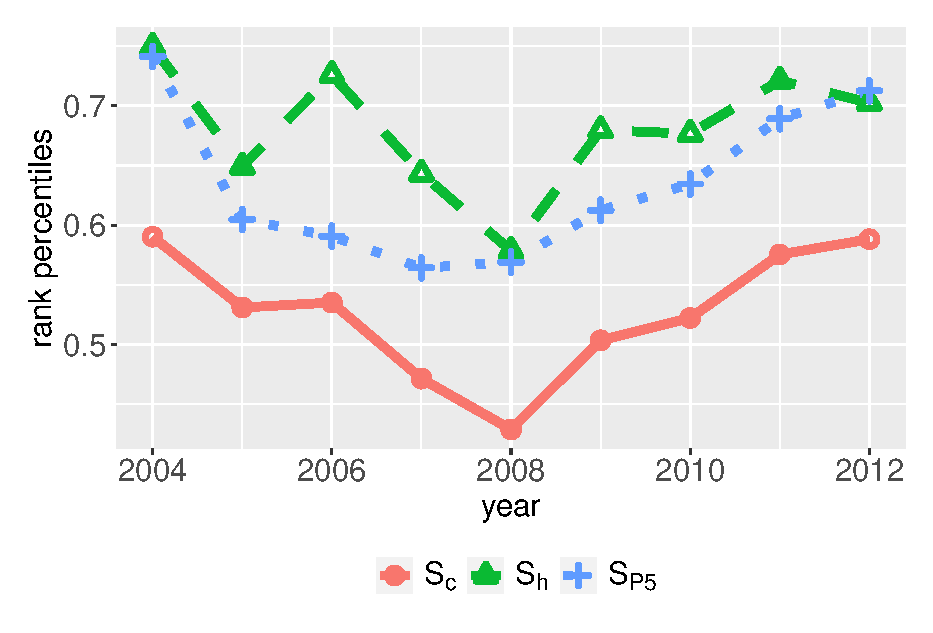
\includegraphics[width=0.6\textwidth]{figures/compare_autrp/auti.eps}
    \caption{{\bf Rank Percentile Indicators for a Random Scholar in the Dataset.} 
    The benchmark is the tenured professors.}
    \label{fig:auti}
\end{figure}

The indicator S$_{P5}$ improves some major drawbacks of S$_c$ and S$_h$. First, it removes the seniority effect of publications. The evaluation metric for S$_c^{i}(t)$ represents the citations that scholar $i$ receives by age $t$, which is the sum of citations for the scholar's publications by $t$. Compared to newly published works, publications with longer histories are more likely to attract citations and therefore provide a greater contribution to formulating S$_c$. A similar argument can be made for S$_h$. However, S$_{P5}$ treats the publications equally and evaluates them based on their performances at the publications' age of 5 years. Additionally, a scholar who publishes a considerable number of low-impact works or participates in only a small number of high-impact projects can have a high value of S$_c$, since the absolute number of citations can be unlimited and is significantly influenced by extreme values. However, the S$_{P5}$ and S$_h$ of these scholars are not necessarily large, since these indicators limit the contribution of a single publication to be, at most, $1$ by definition of rank percentile and h-index score. Furthermore, compared to S$_h$, S$_{P5}$ penalizes scholars who are not truly innovative but carefully massage their h-index scores by publishing a number of papers that attract citation numbers that are barely sufficient to increase their h-index scores. If a paper is among the top $h$ papers, then the actual number of citations is irrelevant for the h-index and S$_h$, but it can still impact S$_{P5}$. Finally, S$_{P5}$ requires less data than S$_c$ and S$_h$, since it only relies on the 5-year citation history of each publication. Hence, S$_{P5}$ is better suited to large-scale analysis.

We demonstrate the advantages of S$_{P5}$ by examining some extreme cases. We considered a benchmark that contains scholars in biology who started their careers in 1990, and we created three synthetic academic careers, adding them to the benchmark just for this experiment. Scholar A publishes a substantial number of publications throughout their career (more papers than $90\%$ of their cohorts in the benchmark), although each of the publications has little impact. Scholars B and C publish only one paper each at the beginning of their careers; B's paper is astonishing, while C's paper is average. Both scholars have an h-index equal to $1$ throughout their careers. Figure \ref{fig:simulated_authors} illustrates the rank percentile indicators for these three artificial scholars. We see that flooding low-impact publications can increase S$_c$ at the beginning of Scholar A's career. Additionally, we see that a single high-impact work improves the value of S$_c$ throughout Scholar B's career; the author remains in the top $50\%$ at age $12$, as indicated by S$_c$. Both S$_{P5}$ and S$_h$ better characterize the performances of these authors. Finally, S$_h$ remains the same for Scholars B and C since they each have an h-index of $1$ throughout their careers. However, S$_{P5}$ considers that Scholar B's publication has a greater impact and therefore ranks Scholar B higher than Scholar C. 

% fig:simulated_authors
% show the difference between various author rp
\begin{figure}[!ht]
    \centering
    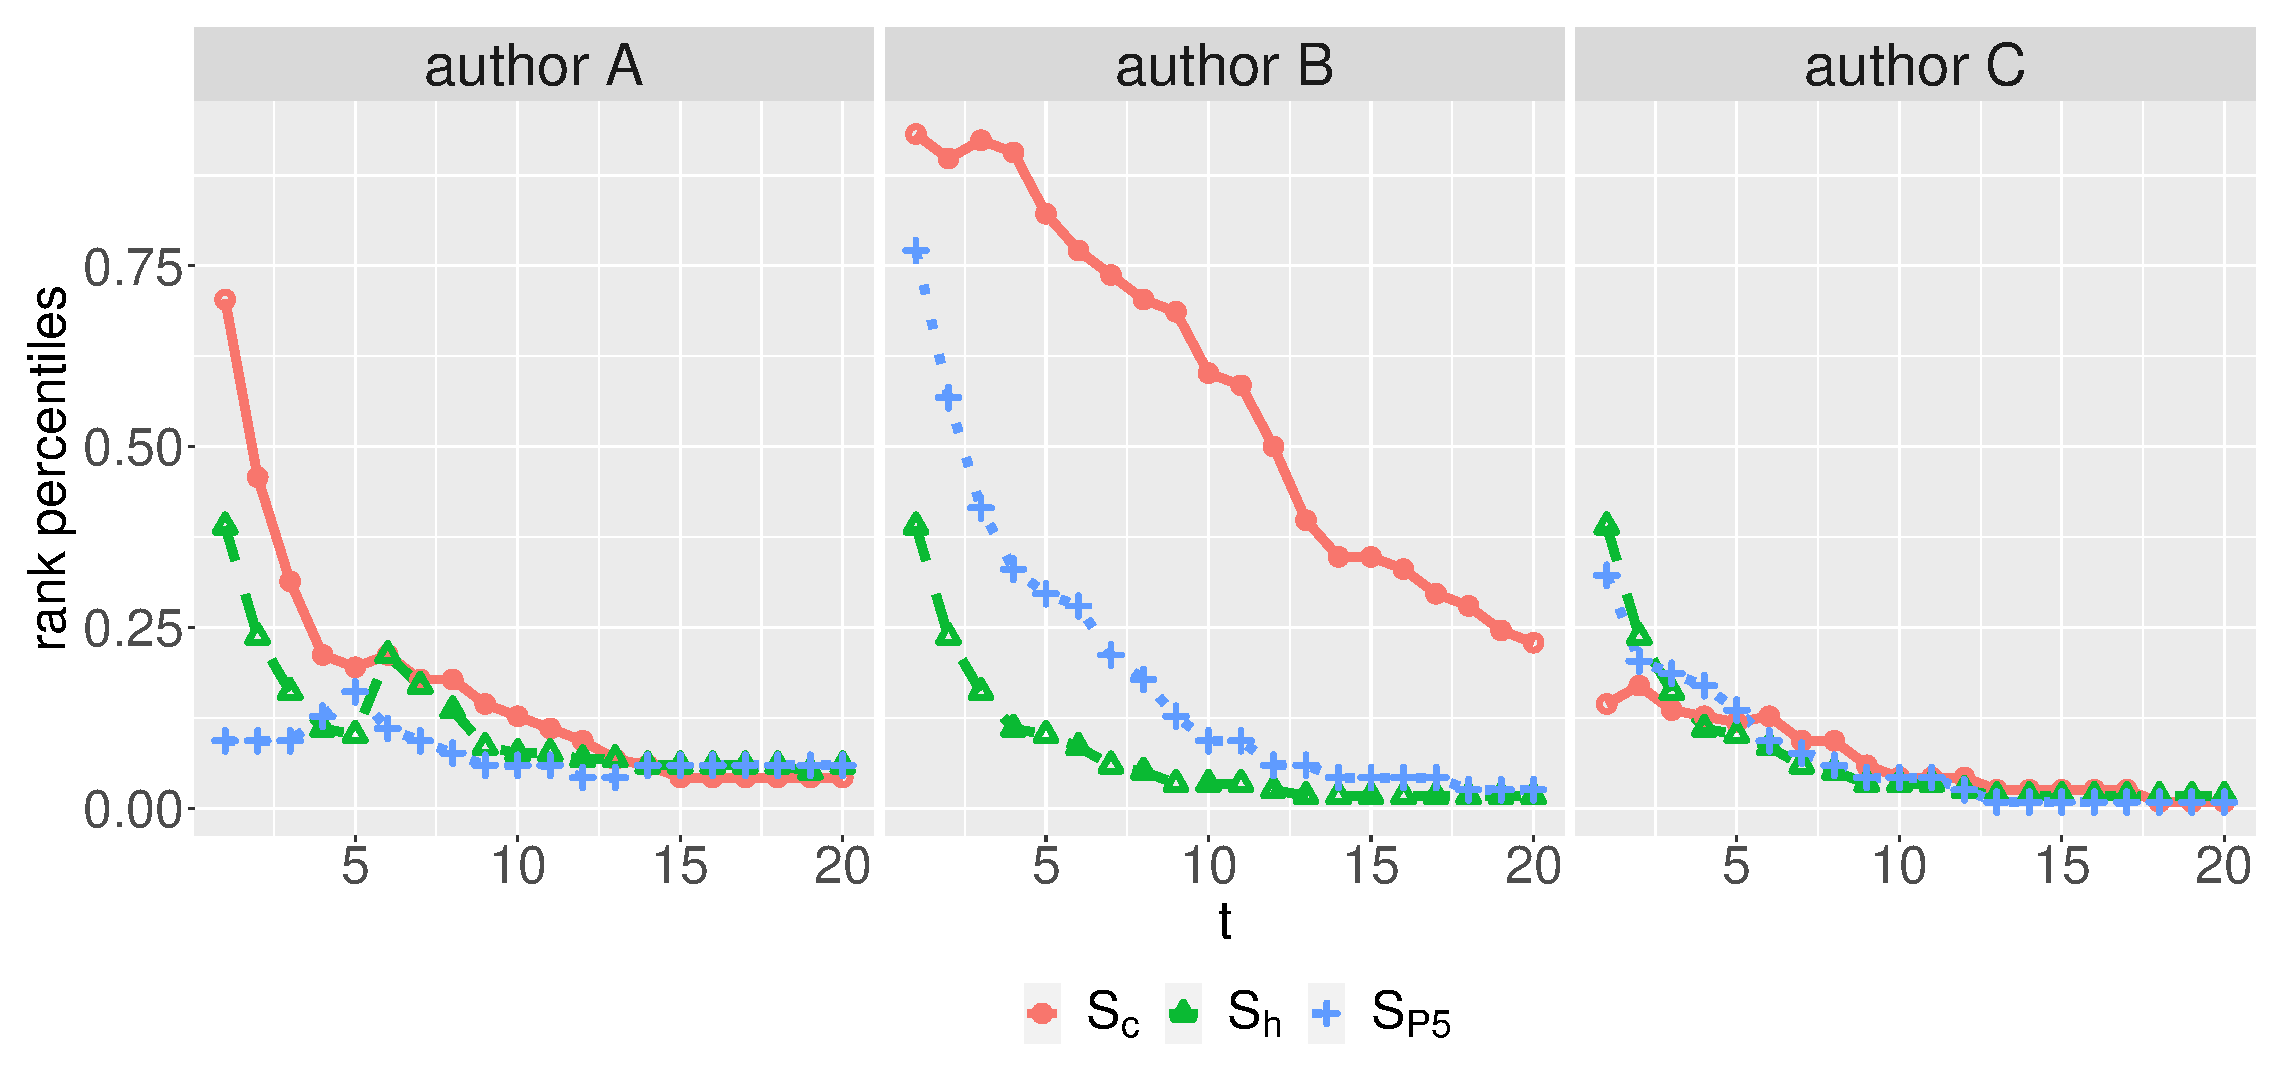
\includegraphics[width=\textwidth]{figures/compare_autrp/simulated_authors.eps}
    \caption{{\bf The Rank Percentile Indicators for Three Artificial Scholars.} The benchmark contains scholars in biology who started their careers in $1990$.}
    \label{fig:simulated_authors}
\end{figure}

With the exception of the above-mentioned discrepancies, we present in the Supplemental Material Section \ref{sec:suppl_similarity_autrp} that for the majority of scholars in our dataset, S$_{P5}$ largely agrees with S$_c$ and S$_h$. Furthermore, we demonstrate the choice of utilizing the 5-year history of a publication. We considered utilizing a longer history (10 years) and found that (as evidenced in the Supplemental Material Section \ref{sec:suppl_robustness_P5}) the differences between the resultant rank percentile indicator and S$_{P5}$ were not statistically significant. A similar conclusion can be obtained by utilizing summary statistics (mean, median, and max) of the rank percentile throughout the entire history of a publication instead of utilizing values at a fixed age, thus indicating the robustness of S$_{P5}$. As we will discuss in the following sections, the publication percentile P$_c^{j}(t)$ is highly stable over $t$, and therefore P$_c^{j}(5)$ is a reasonable indicator of the performance for the publication. Additionally, we sum the rank percentiles for all the publications to obtain the evaluation metric for the scholar. The choice of the sum as the aggregation function considers both the quantity and the quality of the publications, which is in the same spirit of citation counts and h-index values.

\subsection*{The Stationarity of Rank Percentile Indicator}

The rank percentile S$_{P5}$ allows us to compare a scholar with others in the benchmark at a specific age. In the example of the tenure promotion, we compared the 6-year performance of the candidate with the 6-year performance of the senior cohorts. The comparison is not valid if systematic bias exists in which exterior factors, such as the academic environment, result in a better or worse candidate performance than the internal factors, such as creativity and productivity.

Figure \ref{fig:rp_stationarity} portrays S$_{P5}$ at scholar age $10$, grouped by the starting year of academic careers, in which the benchmark is the tenured professors. We see that S$_{P5}$ does not exhibit an obvious upward or downward trend, which would indicate a systematic bias of the indicator that favors junior or senior scholars. The approximate stationarity over the starting year of careers provides empirical evidence for the validity of the rank percentile indicator. 

\begin{figure}[ht!]
    \centering
    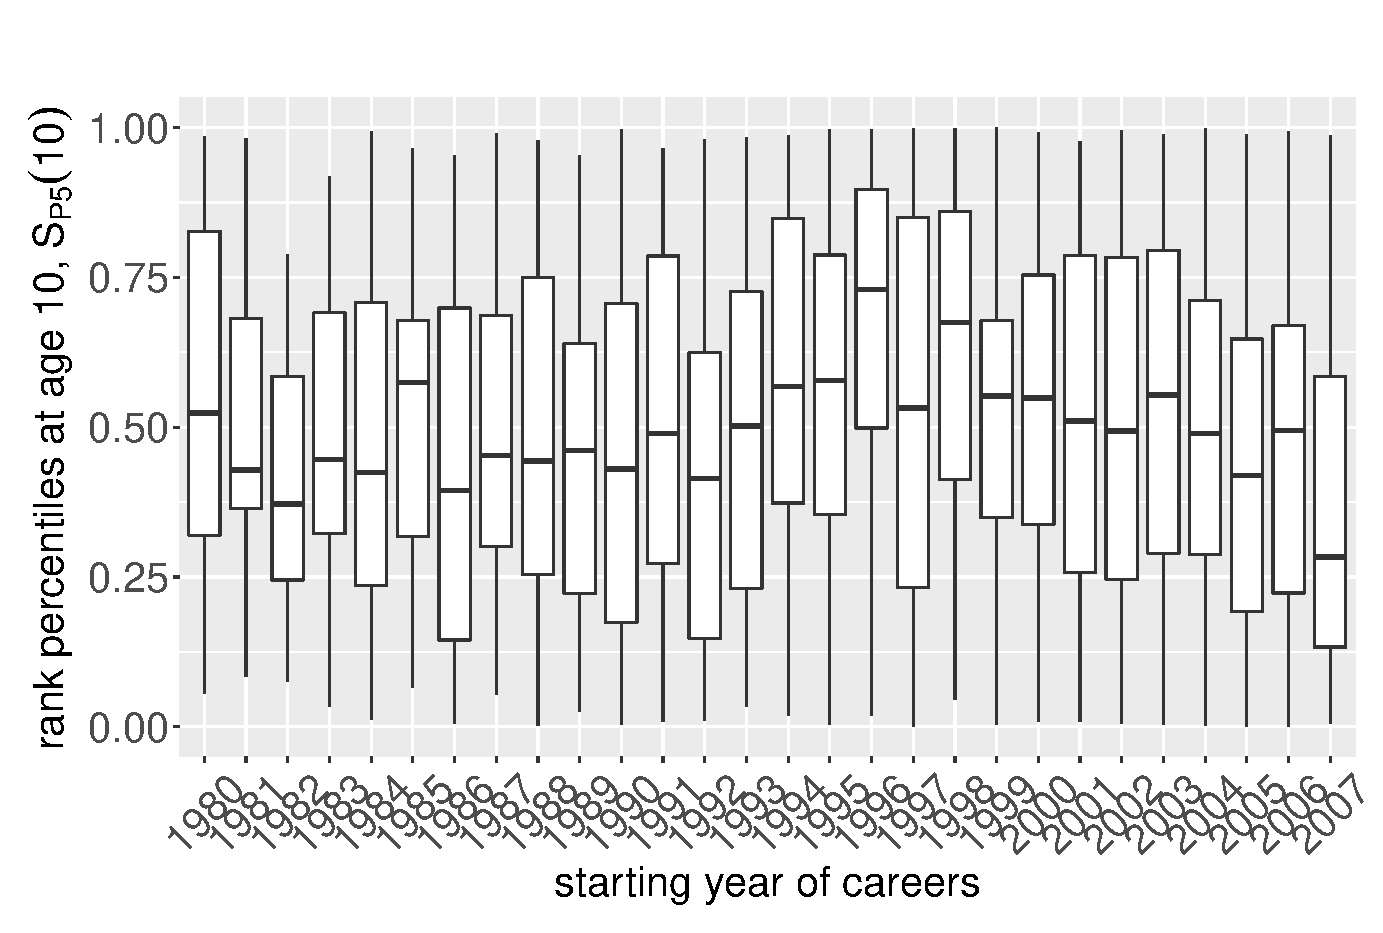
\includegraphics[width=0.6\textwidth]{figures/stationarity/rp_stationarity.eps}
    \caption{{\bf S$_{P5}^i(10)$ Grouped by the Starting Years of Academic Careers.}
    The benchmark is the tenured professors.} 
    \label{fig:rp_stationarity}
\end{figure}

\section*{The Predictability of Rank Percentile Indicator}

Citations have been proven to lack long-term predictive power~\cite{Wang2013}; consider the benchmark of biology as an example. Figure \ref{fig:pred_cit_age} illustrates that papers with the same number of citations by the 5th year since publication can have noticeably different citation paths and long-term effects. Additionally, exceptional and creative ideas typically require a lengthy period to be appreciated by the scientific community. The citation distribution over $30$ years since publication has been proven to have fat tails~\cite{Wang2013}. As presented in Figure \ref{fig:pred_cit_cit}, the correlation between short- (5-year) and long-term (30-year) citations disintegrates for the most highly-cited publications (the shaded rectangle). These problems can be largely avoided by utilizing rank percentile indicators, as evidenced in Figure \ref{fig:pub_rp_pred}. The considerable variation in the long-term effect of citations is restricted by utilizing rank percentiles. For publications with considerable impact, the correlation between short- (5-year) and long-term (30-year) effects persists when utilizing rank percentiles.

% publication rank percentile vs citations, predictability, Wang(2013)
\begin{figure}[ht!]
    \centering
    \begin{subfigure}[b]{0.48\textwidth}
     \centering
     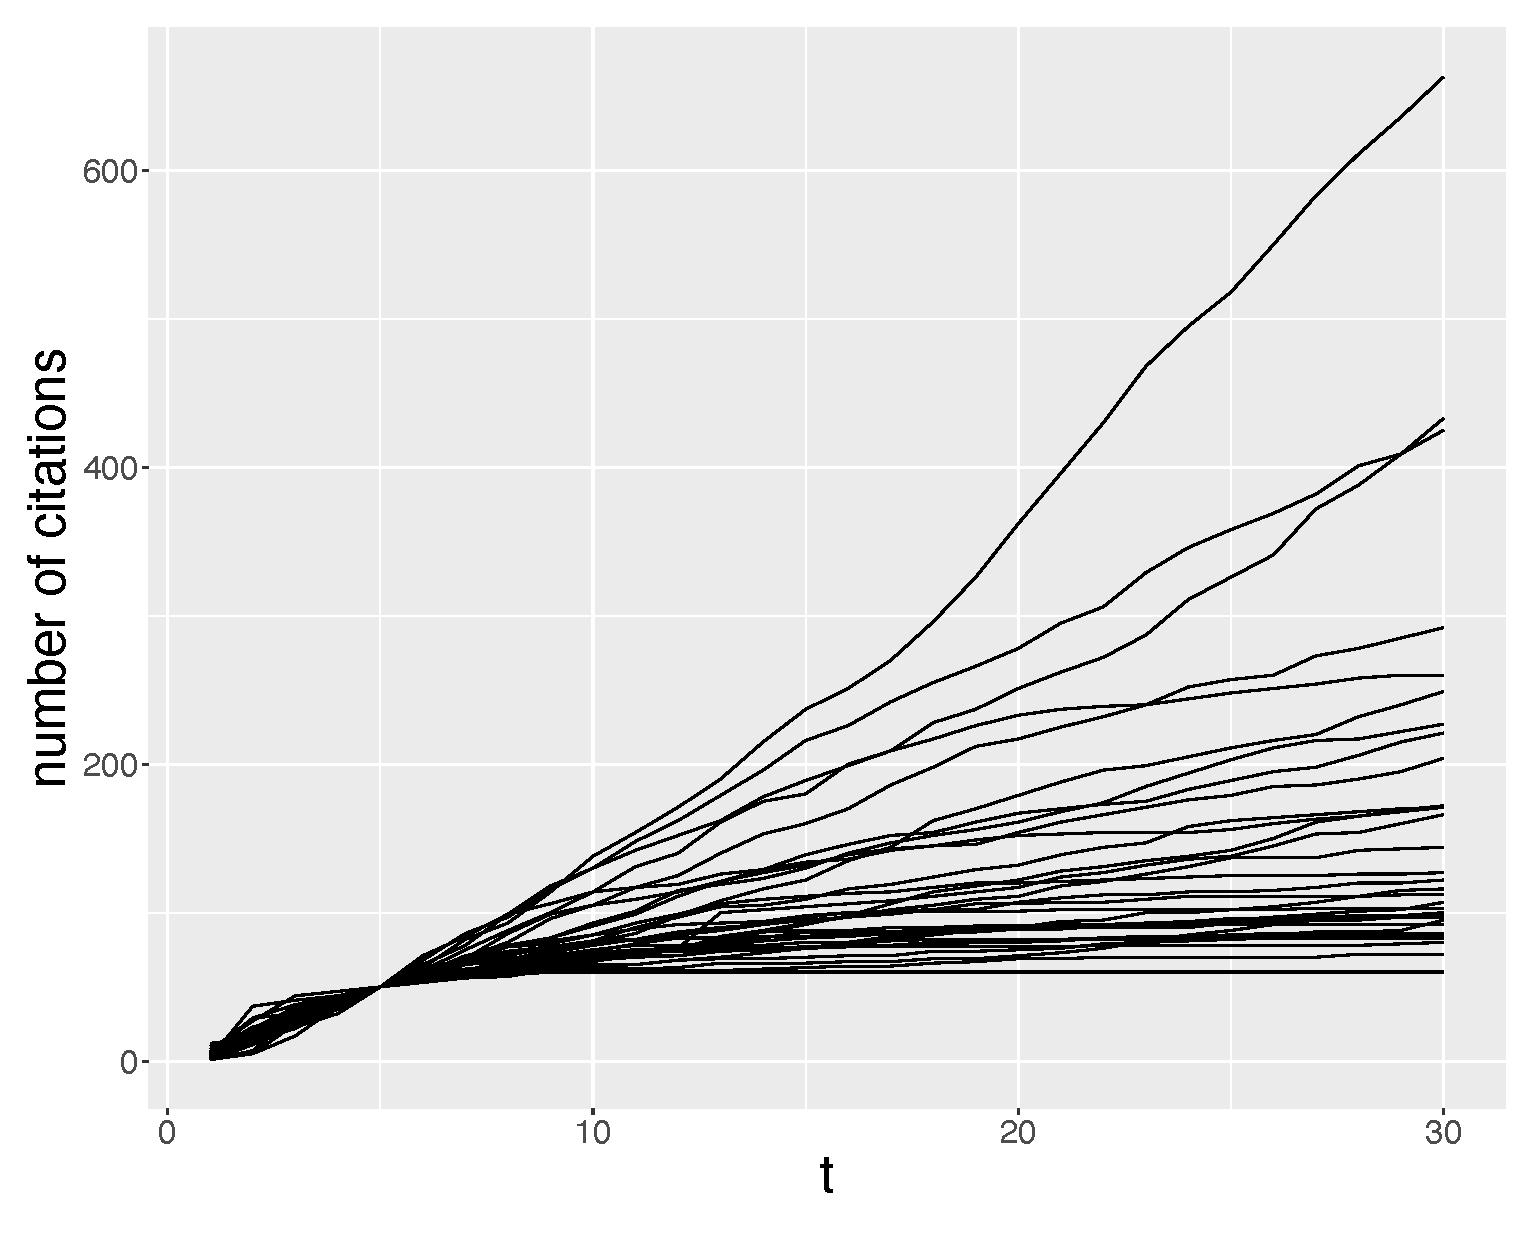
\includegraphics[width=\textwidth]{figures/pred_power/cit_t.eps}
     \caption{Number of citations versus age}
     \label{fig:pred_cit_age}
    \end{subfigure}
    \hfill
    \begin{subfigure}[b]{0.48\textwidth}
     \centering
     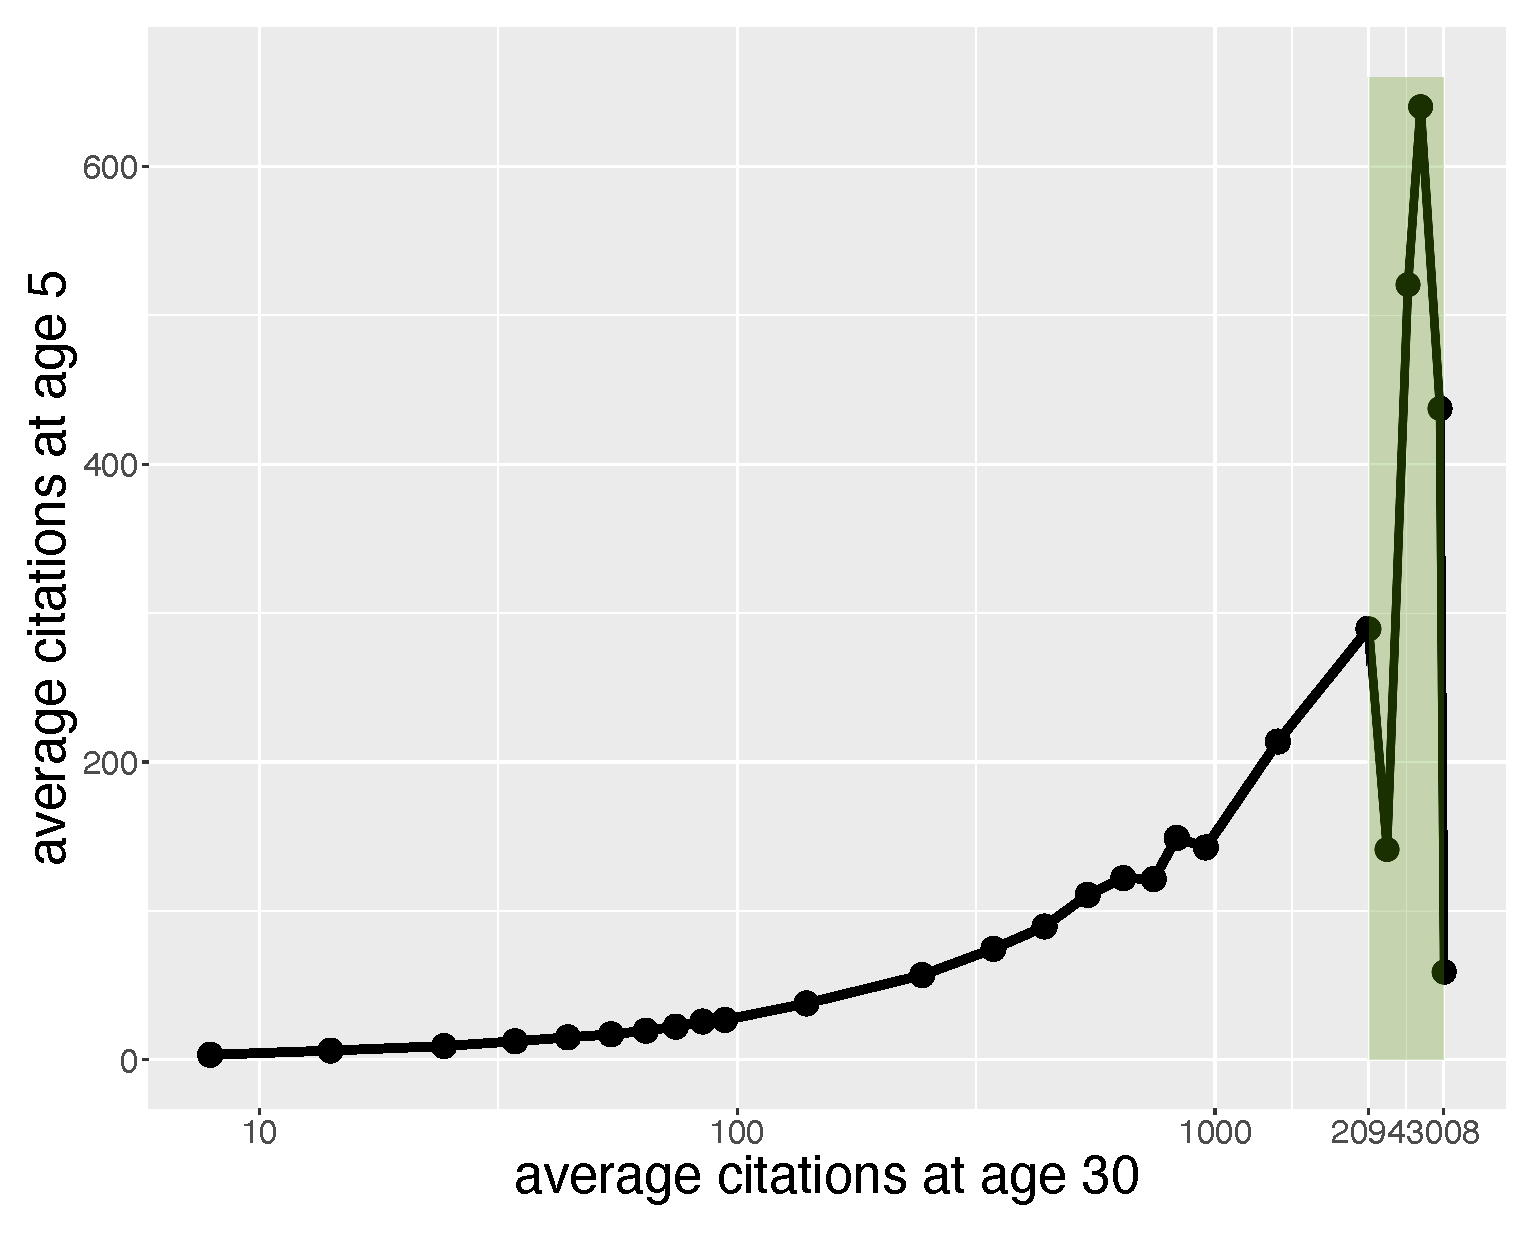
\includegraphics[width=\textwidth]{figures/pred_power/cit_cit.eps}
     \caption{Average citations at age $5$ versus those at age $30$}
     \label{fig:pred_cit_cit}
    \end{subfigure}
    \caption{{\bf Predictability of Citations.}
    The benchmark is the field of biology. Figure \ref{fig:pred_cit_age} portrays the cumulative citations for publications that have $50$ citations by the 5th year since publication. Figure \ref{fig:pred_cit_cit} displays the average citations by age $5$ versus the average citations by age $30$. The averages are calculated over groups of publications, which are prespecified by dividing the range of citations by age $30$ into equal intervals on the log scale. Note that we do not claim the originality of the figures, which have been illustrated via a different dataset~\cite{Wang2013}.}
    \label{fig:pub_cit_pred}
\end{figure}


\begin{figure}[ht!]
    \centering
    \begin{subfigure}[b]{0.495\textwidth}
     \centering
     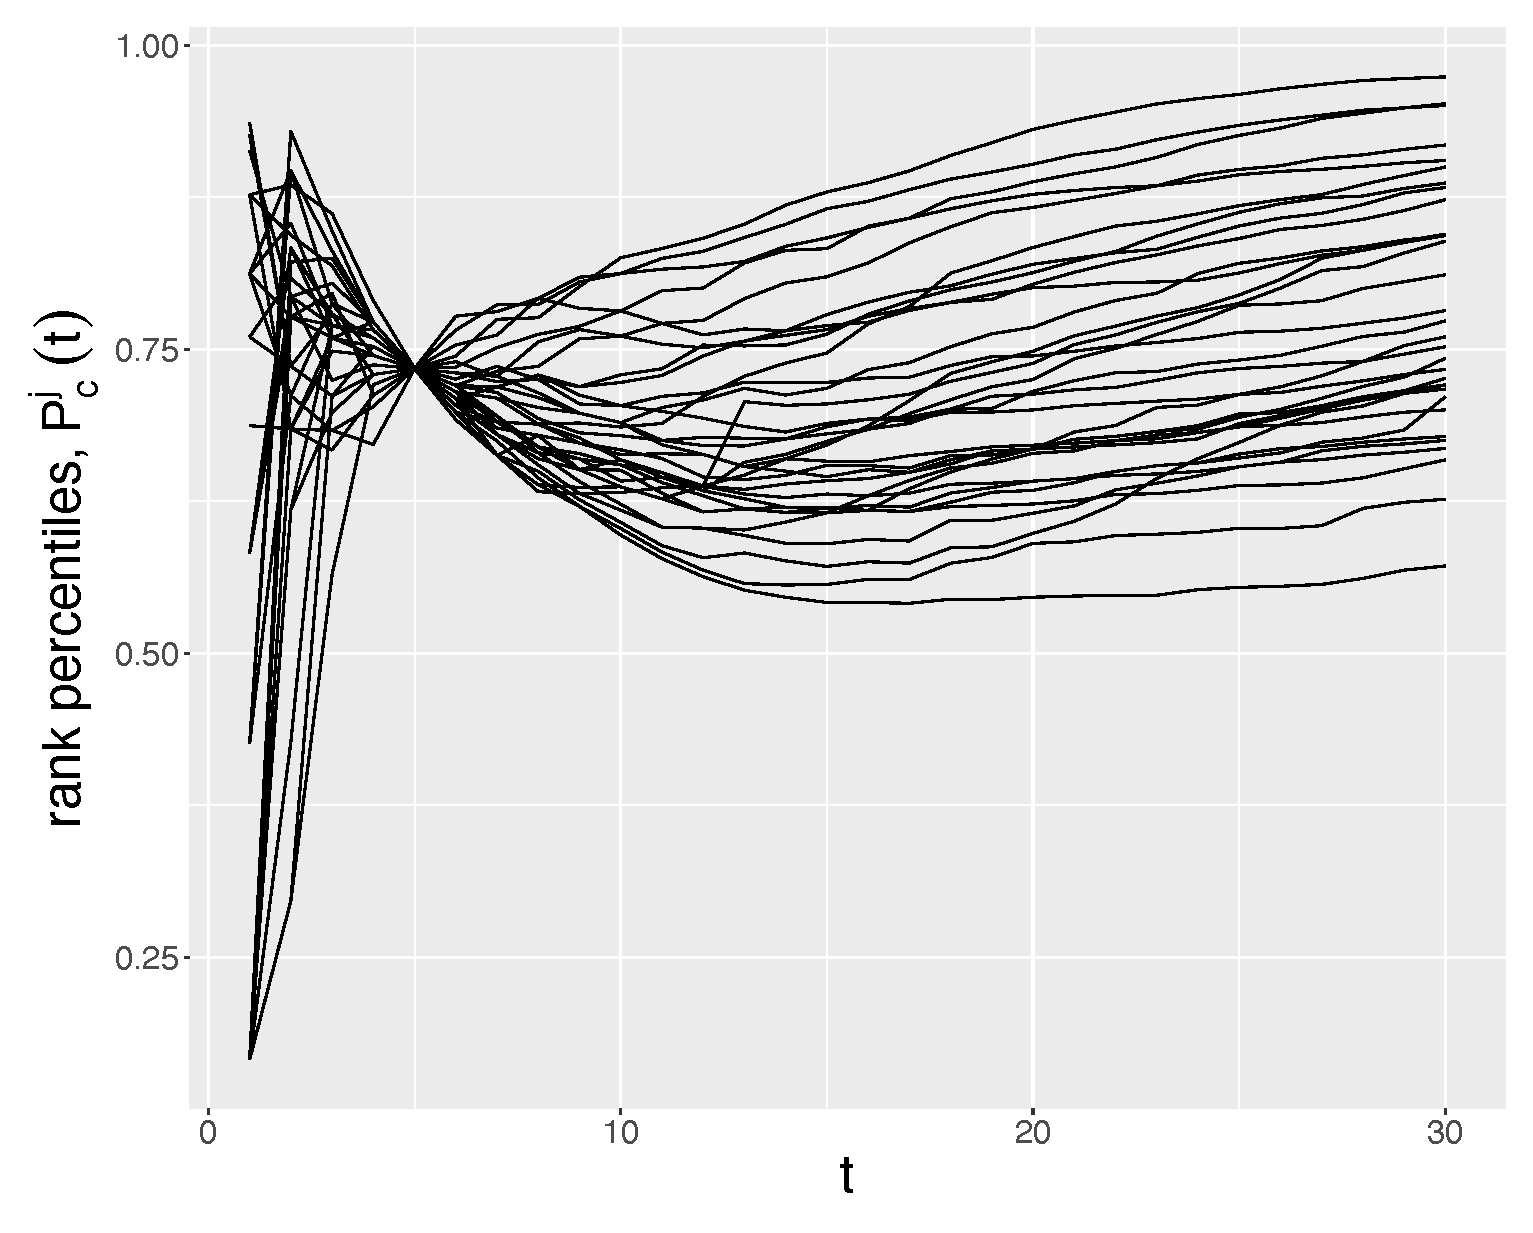
\includegraphics[width=\textwidth]{figures/pred_power/rp_t.eps}
     \caption{Rank percentiles P$_c$ versus age}
     \label{fig:pred_rp_age}
    \end{subfigure}
    \hfill
    \begin{subfigure}[b]{0.495\textwidth}
     \centering
     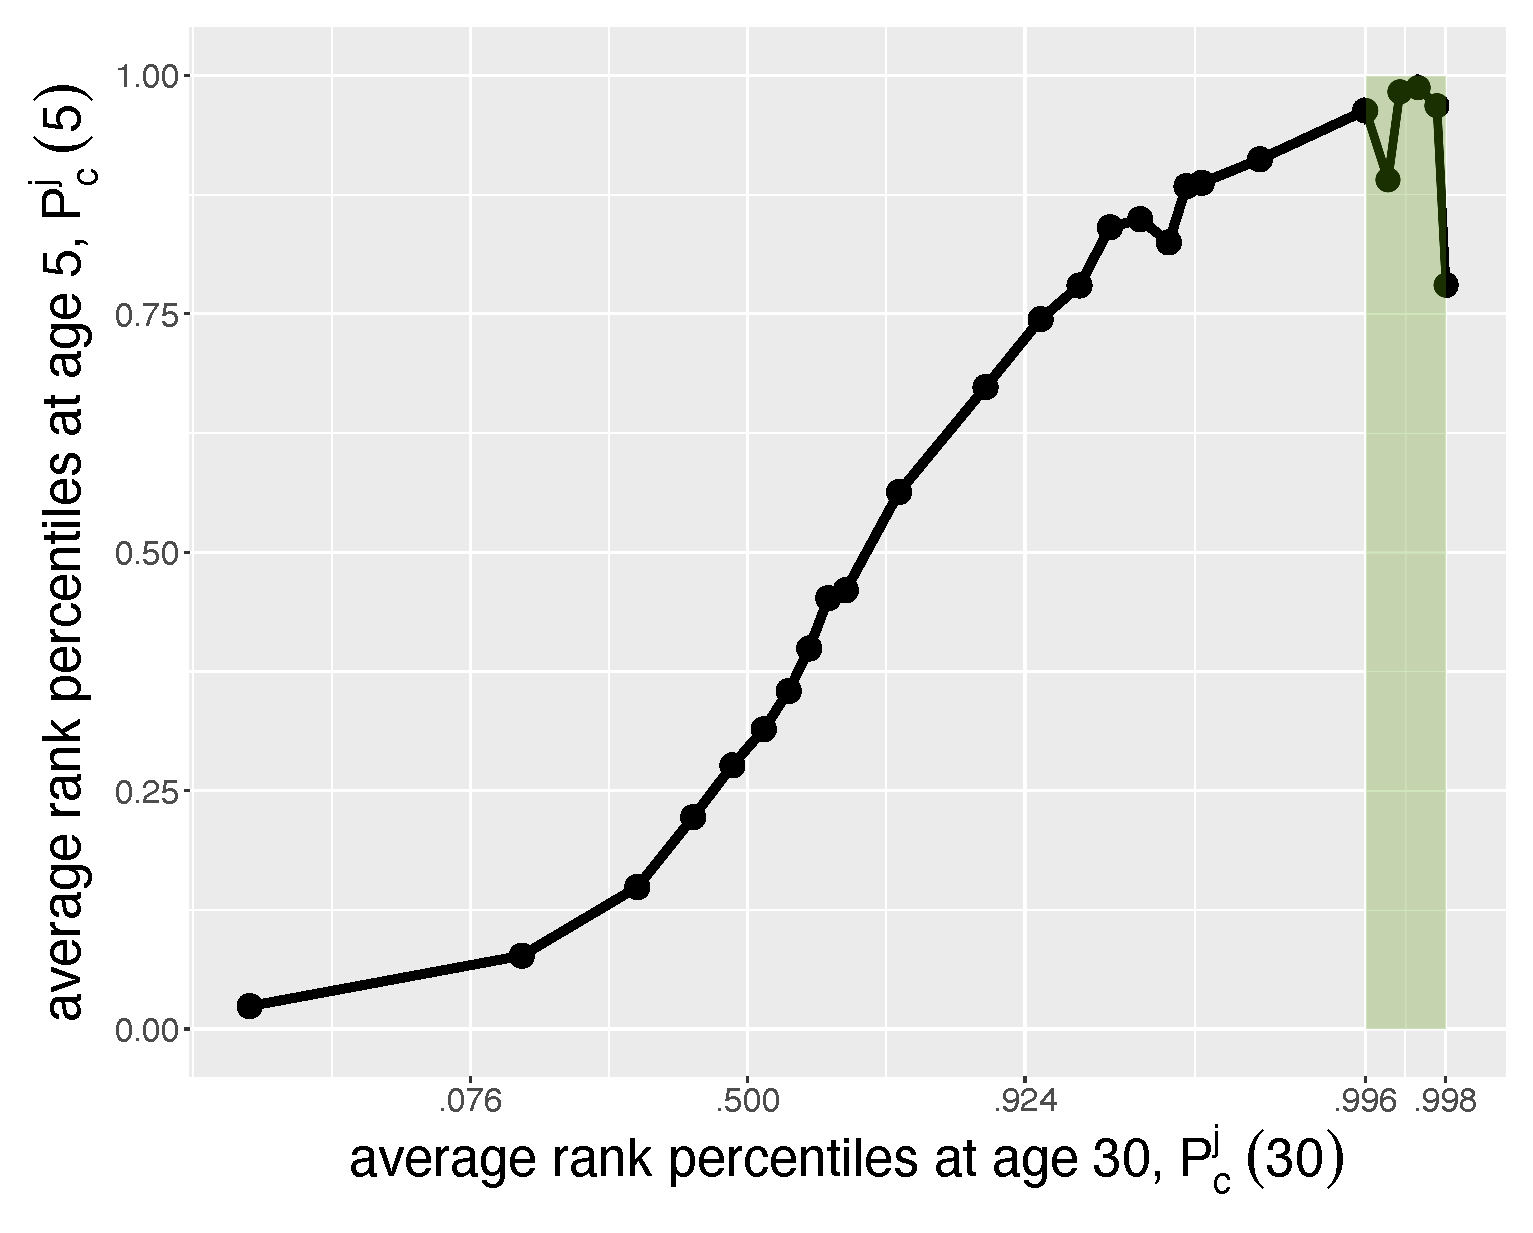
\includegraphics[width=\textwidth]{figures/pred_power/rp_rp.eps}
     \caption{Average P$_c$ at age $5$ versus those at age $30$}
     \label{fig:pred_rp_rp}
    \end{subfigure}
    \caption{{\bf Predictability of Rank Percentiles.}
    Figure \ref{fig:pred_rp_age} demonstrates the rank percentiles for the publications considered in Figure \ref{fig:pred_cit_age}. Figure \ref{fig:pred_rp_rp} presents the average of P$^j_c(5)$ versus the average of P$^j_c(30)$ for the same groups of publications as in Figure \ref{fig:pred_cit_cit}.}
    \label{fig:pub_rp_pred}
\end{figure}

We further characterize the predictability of rank percentile indicators. Figure \ref{fig:hm_rp_pub} presents the Pearson correlation between rank percentiles at two ages, P$_c^{j}(t_1)$ and P$_c^{j}(t_2)$ where $t_1<t_2$. Overall, we noticed large correlations for both benchmarks. The correlation diminishes as the forecast horizon $(t_2-t_1)$ increases, which simply reflects the difficulty of long-term forecasting. Additionally, the correlation increases as $t_1$ increases when the forecast horizon is fixed. This indicates that the performance of a senior publication is easier to predict, since the longer history removes more uncertainties regarding its performance. We further noticed a slightly higher predictive power when we restricted the benchmark to biology. 

% publication rank percentile, heat map of correlations
\begin{figure}[ht!]
    \centering
    \begin{subfigure}[b]{0.8\textwidth}
        \centering
             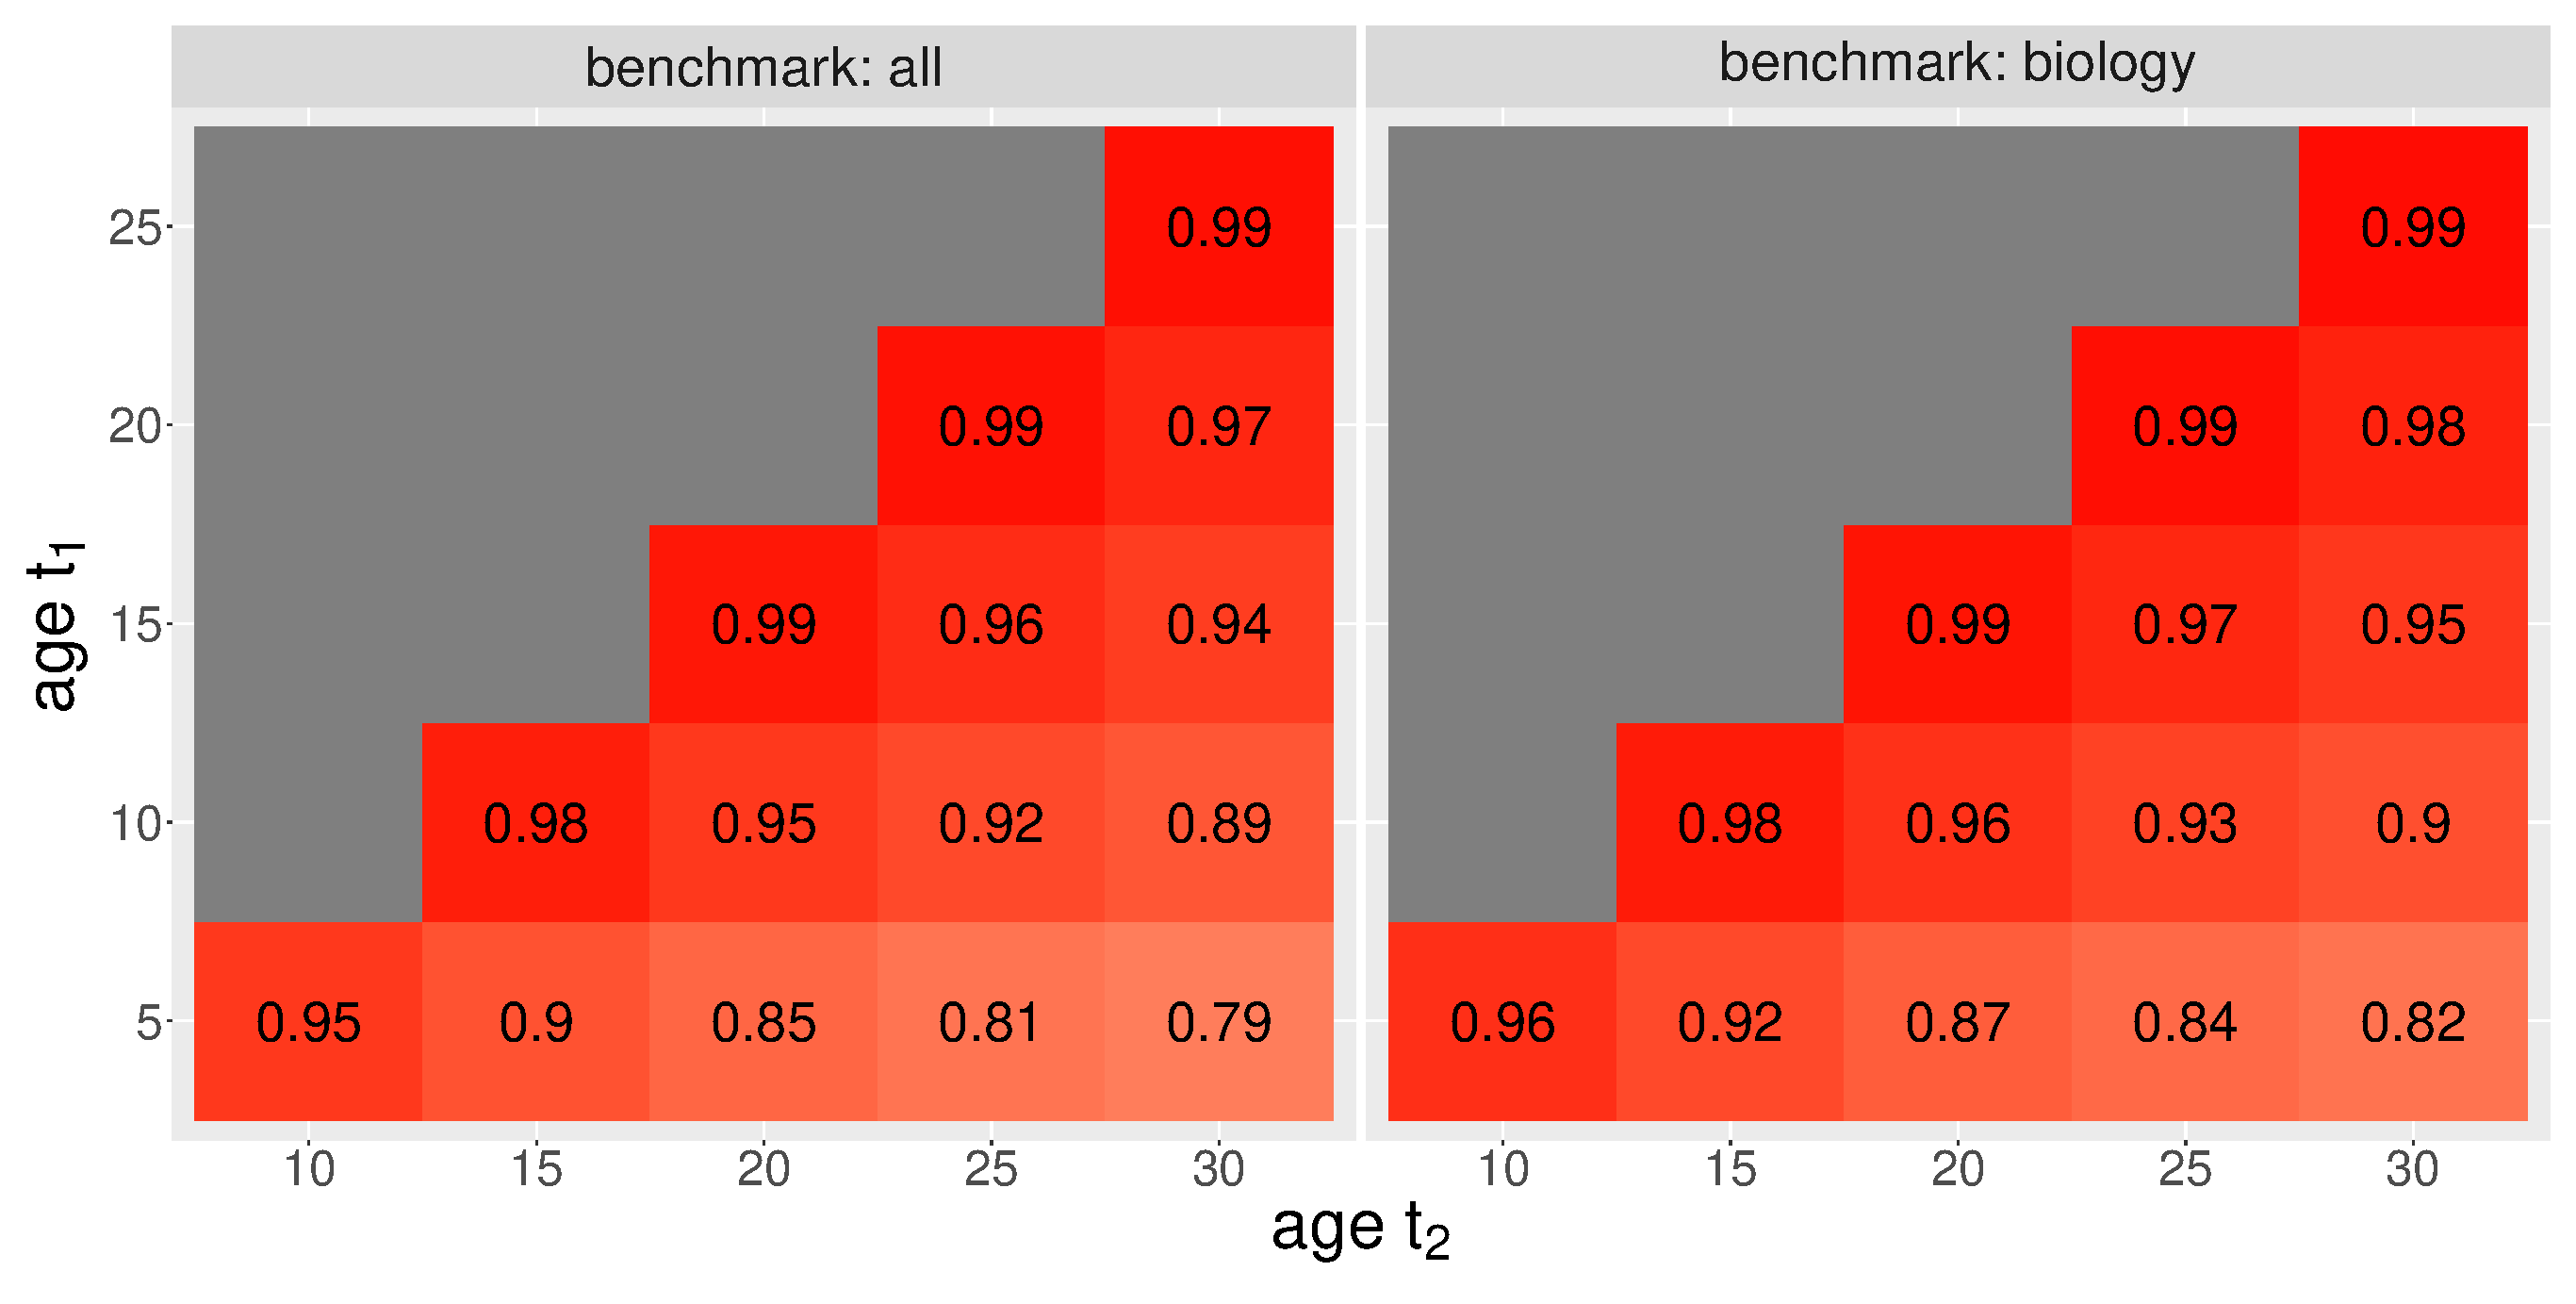
\includegraphics[width=\textwidth]{figures/pred_power/heatmap_cor_pub.eps}
         \caption{Correlation between P$_c^{j}(t_1)$ and P$_c^{j}(t_2)$}
         \label{fig:hm_rp_pub}
    \end{subfigure}

    \begin{subfigure}[b]{0.8\textwidth}
        \centering
             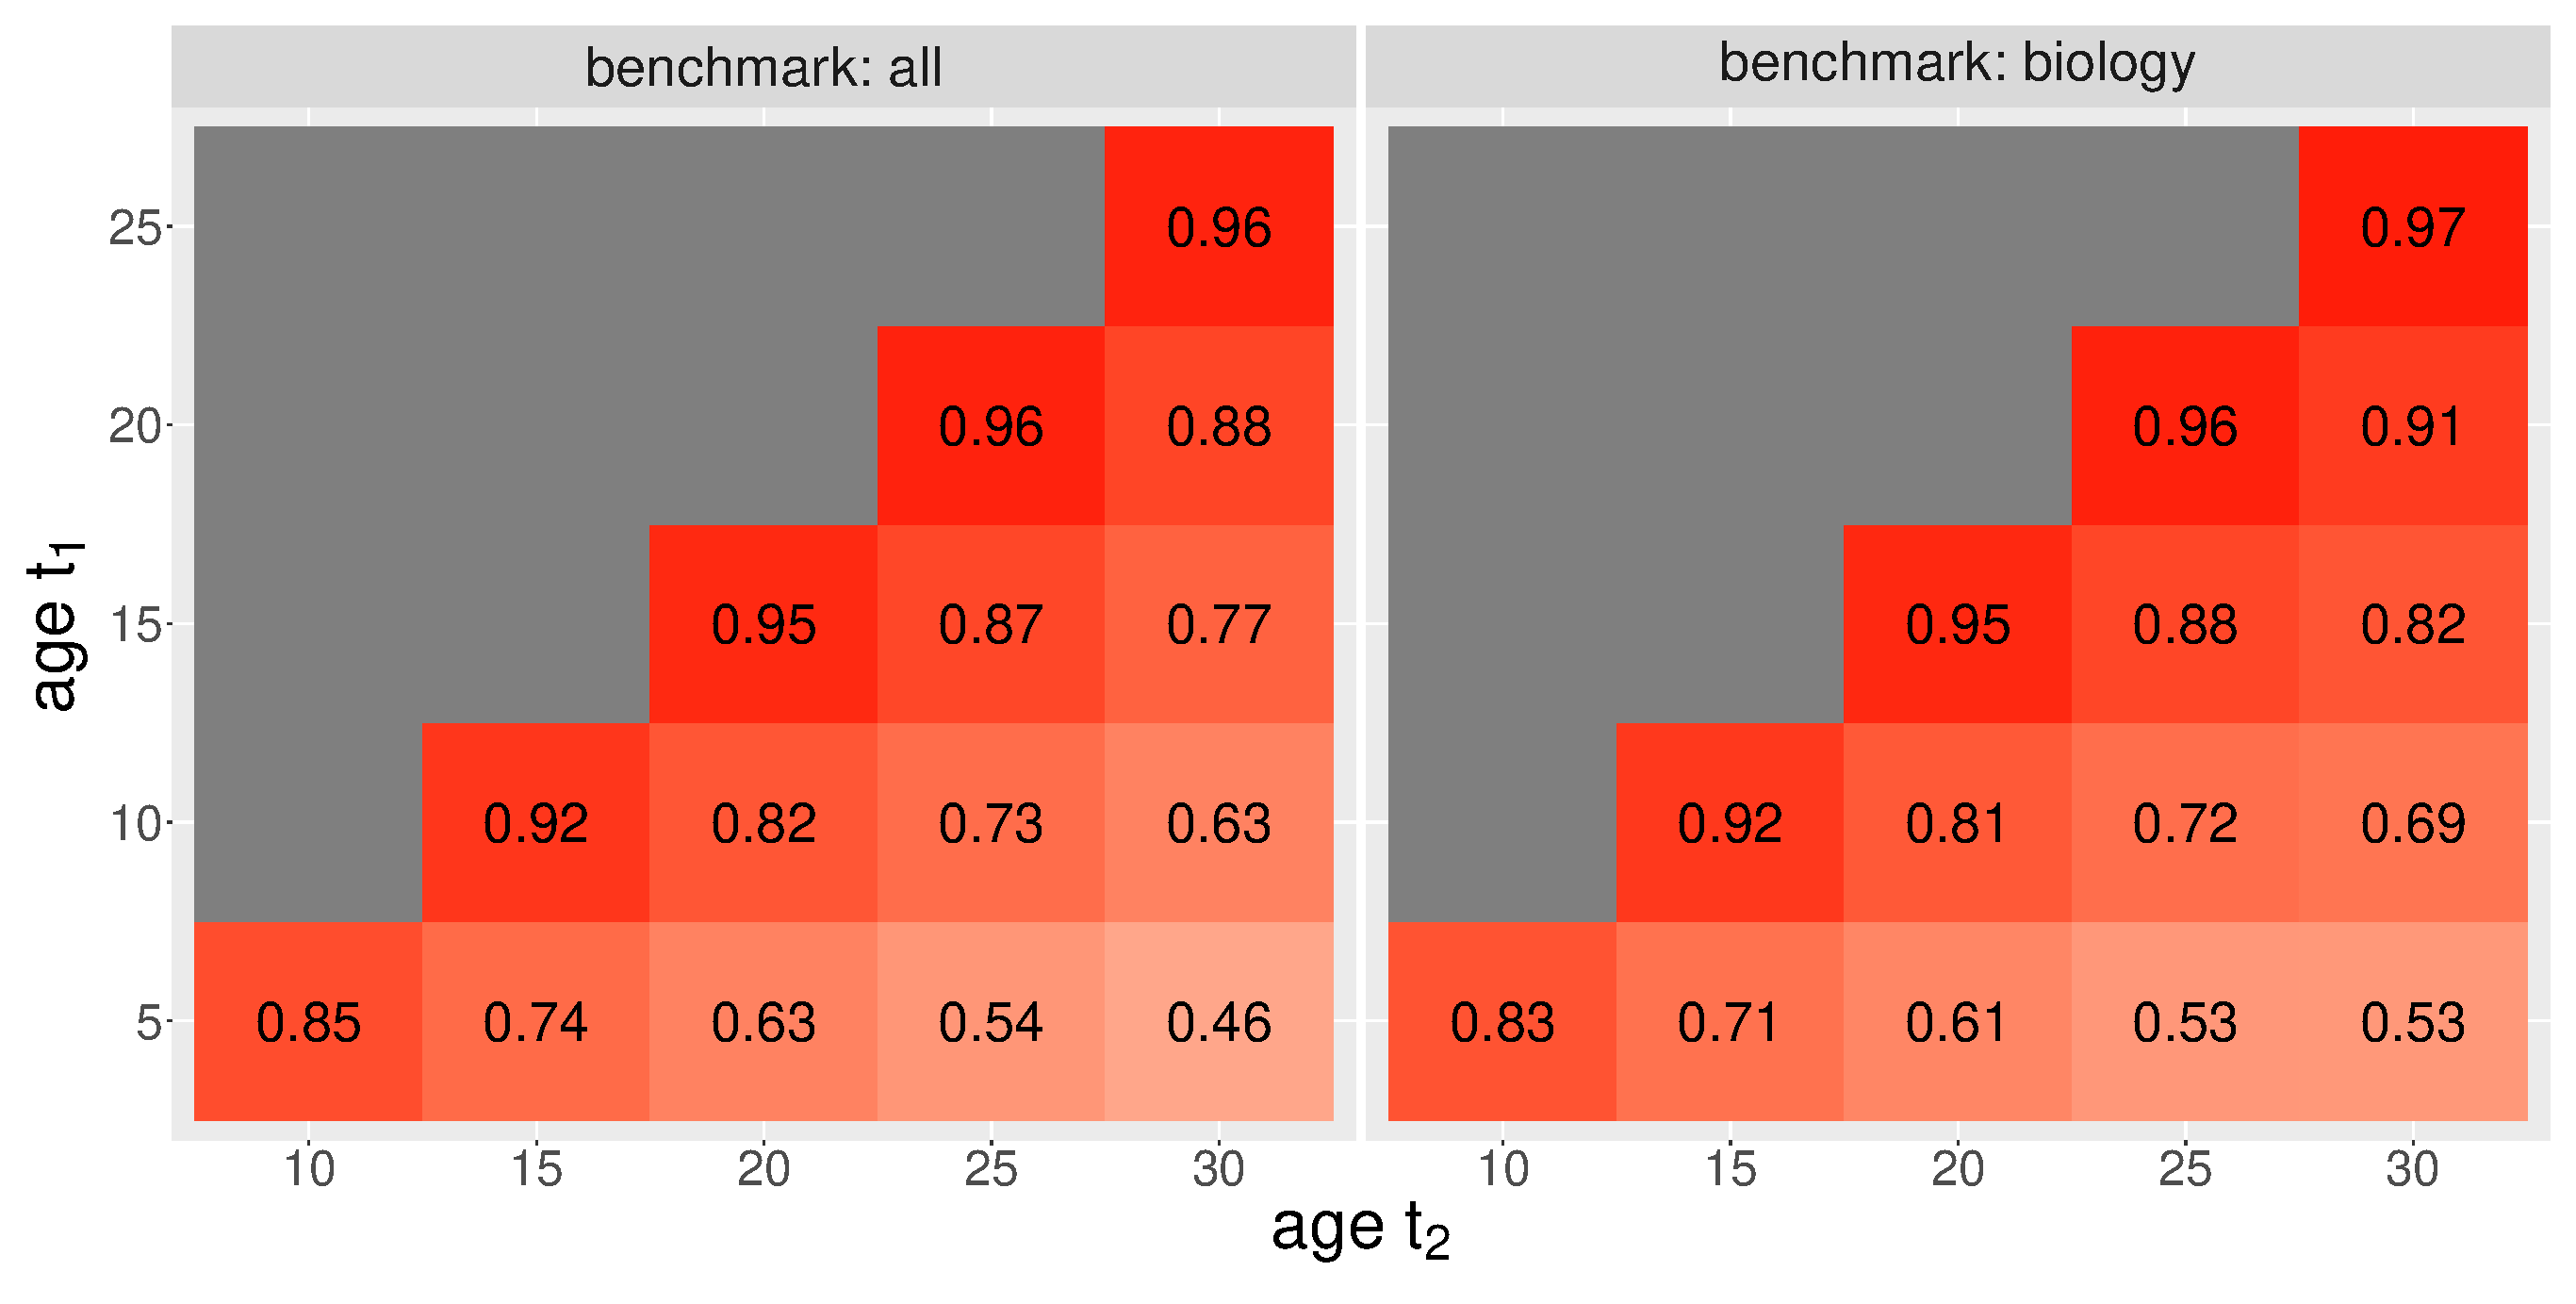
\includegraphics[width=\textwidth]{figures/pred_power/heatmap_cor_aut.eps}
         \caption{Correlation between S$_{P5}^{i}(t_1)$ and S$_{P5}^{i}(t_2)$}
         \label{fig:hm_rp_aut}
    \end{subfigure}

    \begin{subfigure}[b]{0.8\textwidth}
        \centering
             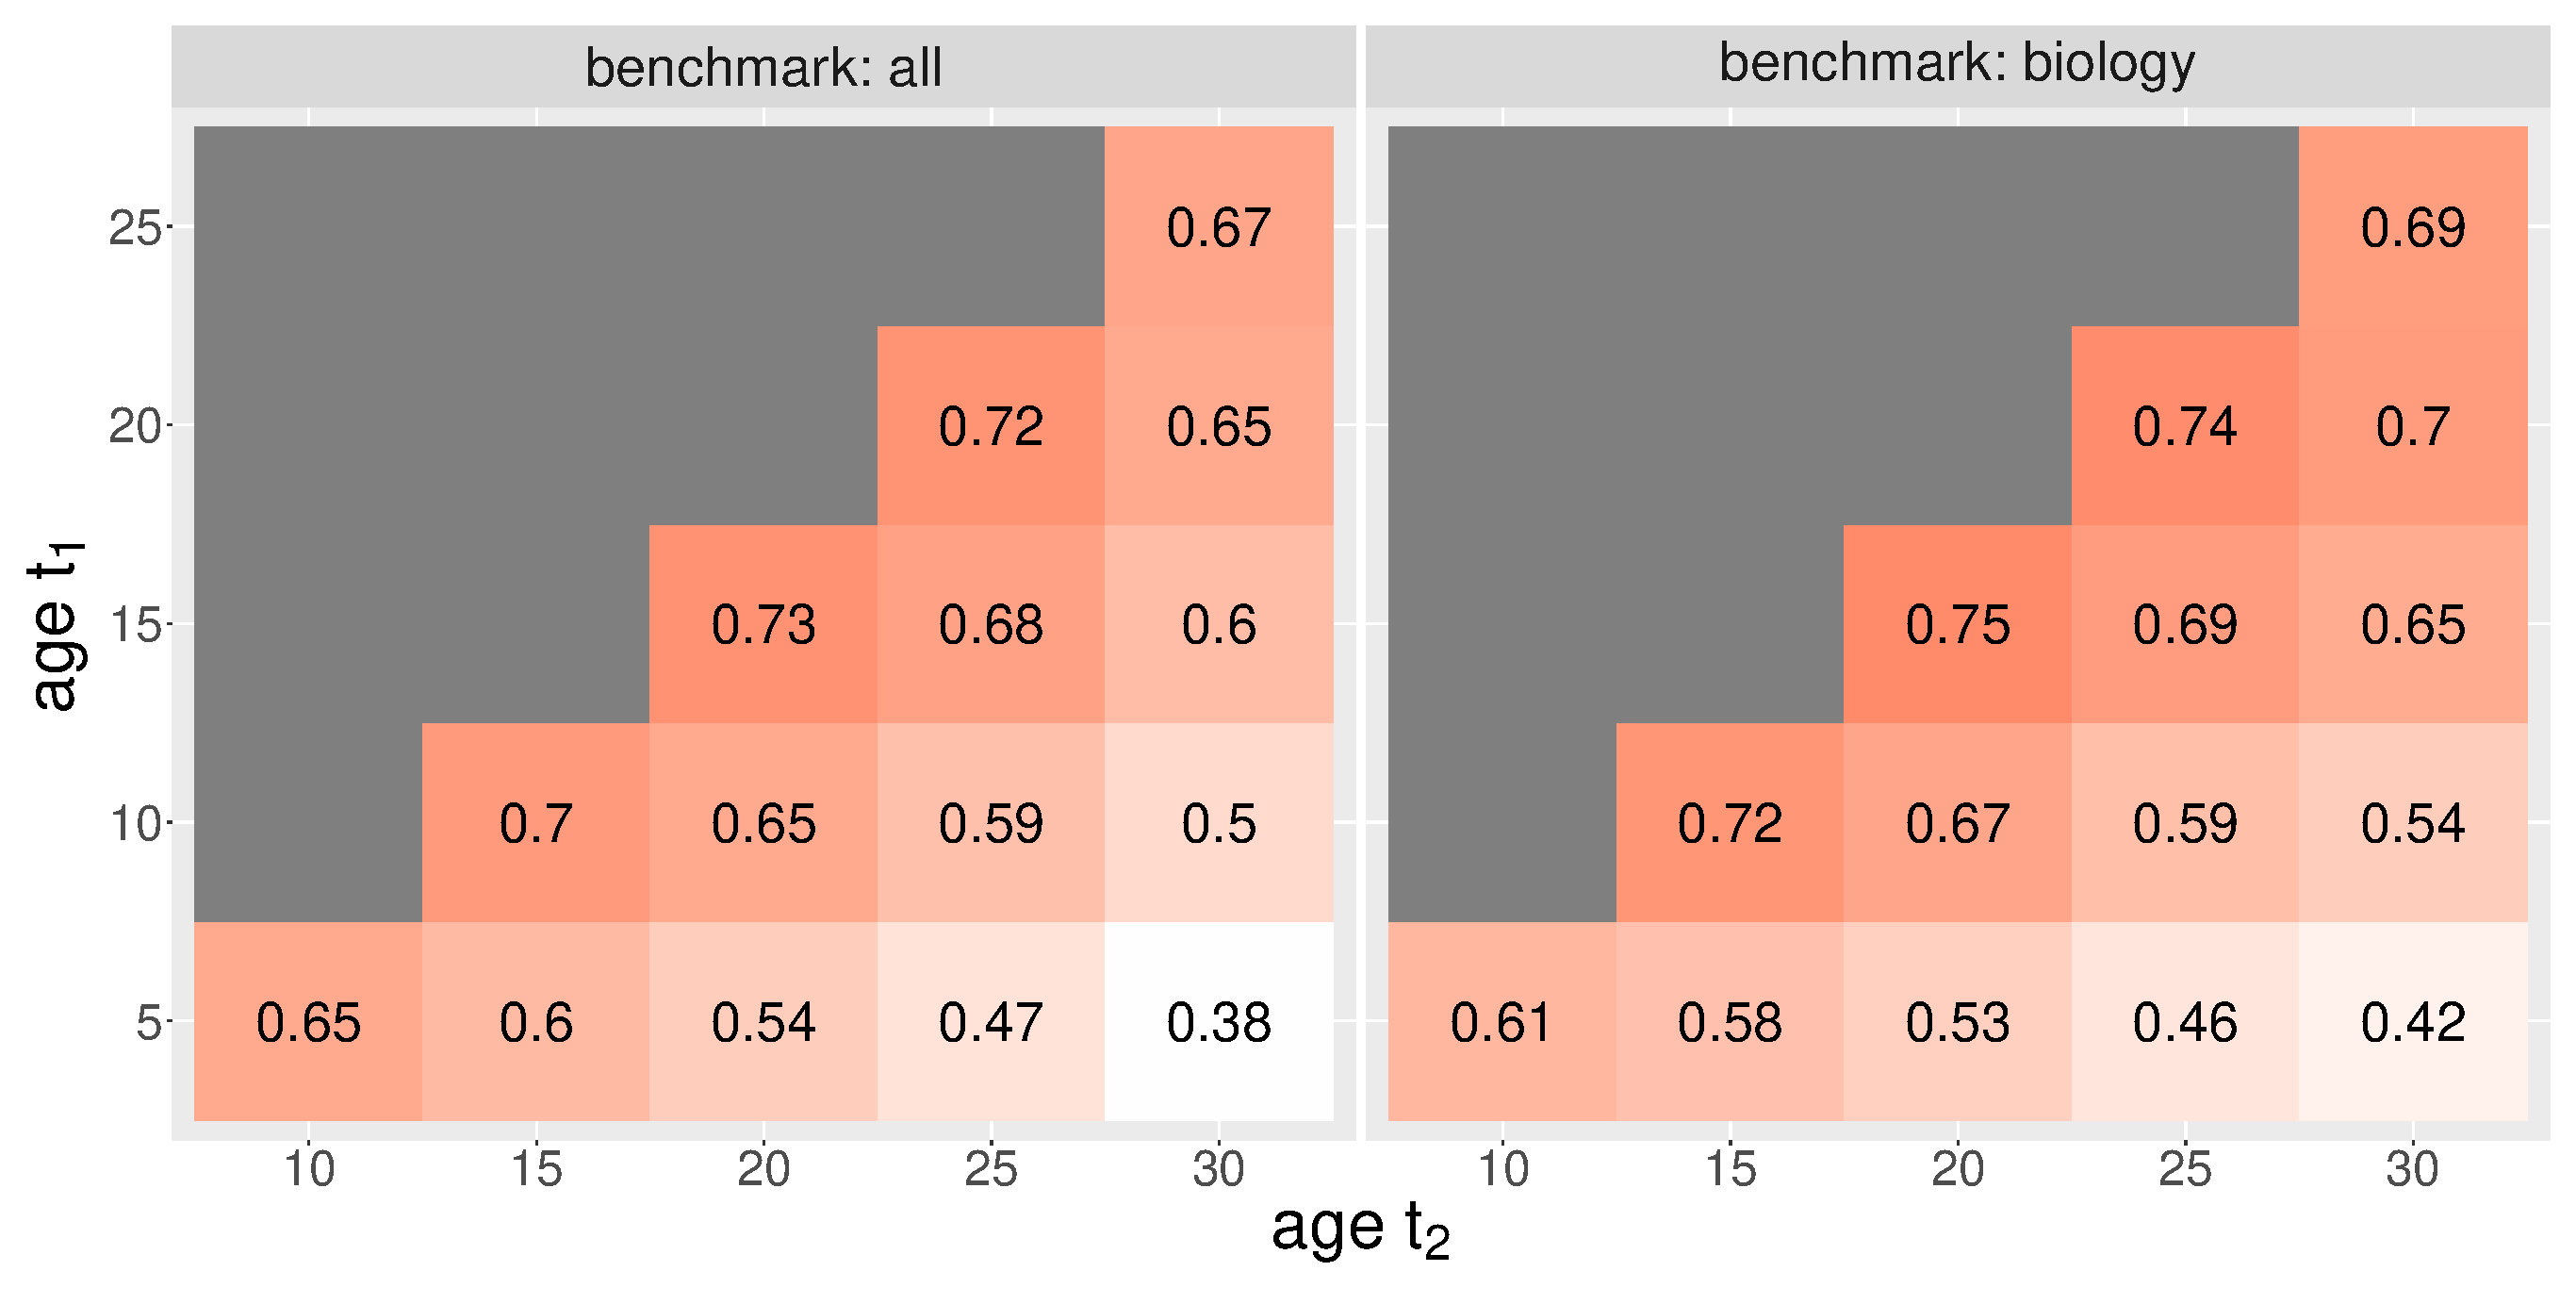
\includegraphics[width=\textwidth]{figures/pred_power/heatmap_cor_aut_future.eps}
         \caption{Correlation between S$_{P5}^{i}(t_1)$ and S$_{P5}^{i}(t_2 | t_1)$}
         \label{fig:hm_rp_aut_future}
    \end{subfigure}
    \caption{{\bf Pearson Correlation between Rank Percentiles at Different Ages.} The benchmark is either all or biology, and it is specified in each of the subfigures.}
    \label{fig:hm_rp}
\end{figure}

Figure \ref{fig:hm_rp_aut} illustrates that the patterns discussed above generally hold for S$_{P5}$. However, the magnitude of correlations is smaller than those for publications, especially for long-term forecasts, because forecasting the future impact of future works is considerably more difficult than forecasting the future impact of existing works. The percentile S$_{P5}^{i}(t_2)$ is based on papers published before $t_2$, which can be divided into papers published before $(t_1-5)$, between $(t_1-5)$ and $t_1$, and between $t_1$ and $t_2$. Since we utilized P$_c^{j}(5)$ (the publication rank percentile by 5 years since publication) to evaluate each publication, the performance of papers published before $(t_1-5)$ was represented by $t_1$. Predicting the performance of papers published between $(t_1-5)$ and $t_1$ is thus predicting the future impact of existing works, while predicting the performance of those published between $t_1$ and $t_2$ is predicting the future impact of future works. However, predicting the publication indicator P$_c^{j}(t_2)$ involves predicting only the future impact of publication $j$, which is a considerably easier task. Additionally, when the forecast horizon increases while $t_1$ is fixed, additional future works are involved in predicting S$_{P5}^{i}(t_2)$; therefore, we see that the correlation decreases more quickly than when we predict P$_c^{j}(t_2)$. 

The strong linear relationship between P$_{c}^{j}(t_1)$ and P$_c^{j}(t_2)$ is further characterized in Figure \ref{fig:scatter_pubrp_bio1980}, where we restricted, for a better visualization, the benchmark to be the publications in biology that were published in $1980$. The data are along the $45 \degree$ line, and the linear regression coefficient of P$_c^{j}(t_2)$ on P$_c^{j}(t_1)$ is close to $1$ with small standard errors, thus indicating the high stability of P$_c$ over time $t$. A similar figure for S$_{P5}$ is displayed in the Supplemental Material Figure \ref{fig:scatter_autrp_all}, in which we find that S$_{P5}$ exhibits short-term stability.


\begin{figure}[ht!]
    \centering
    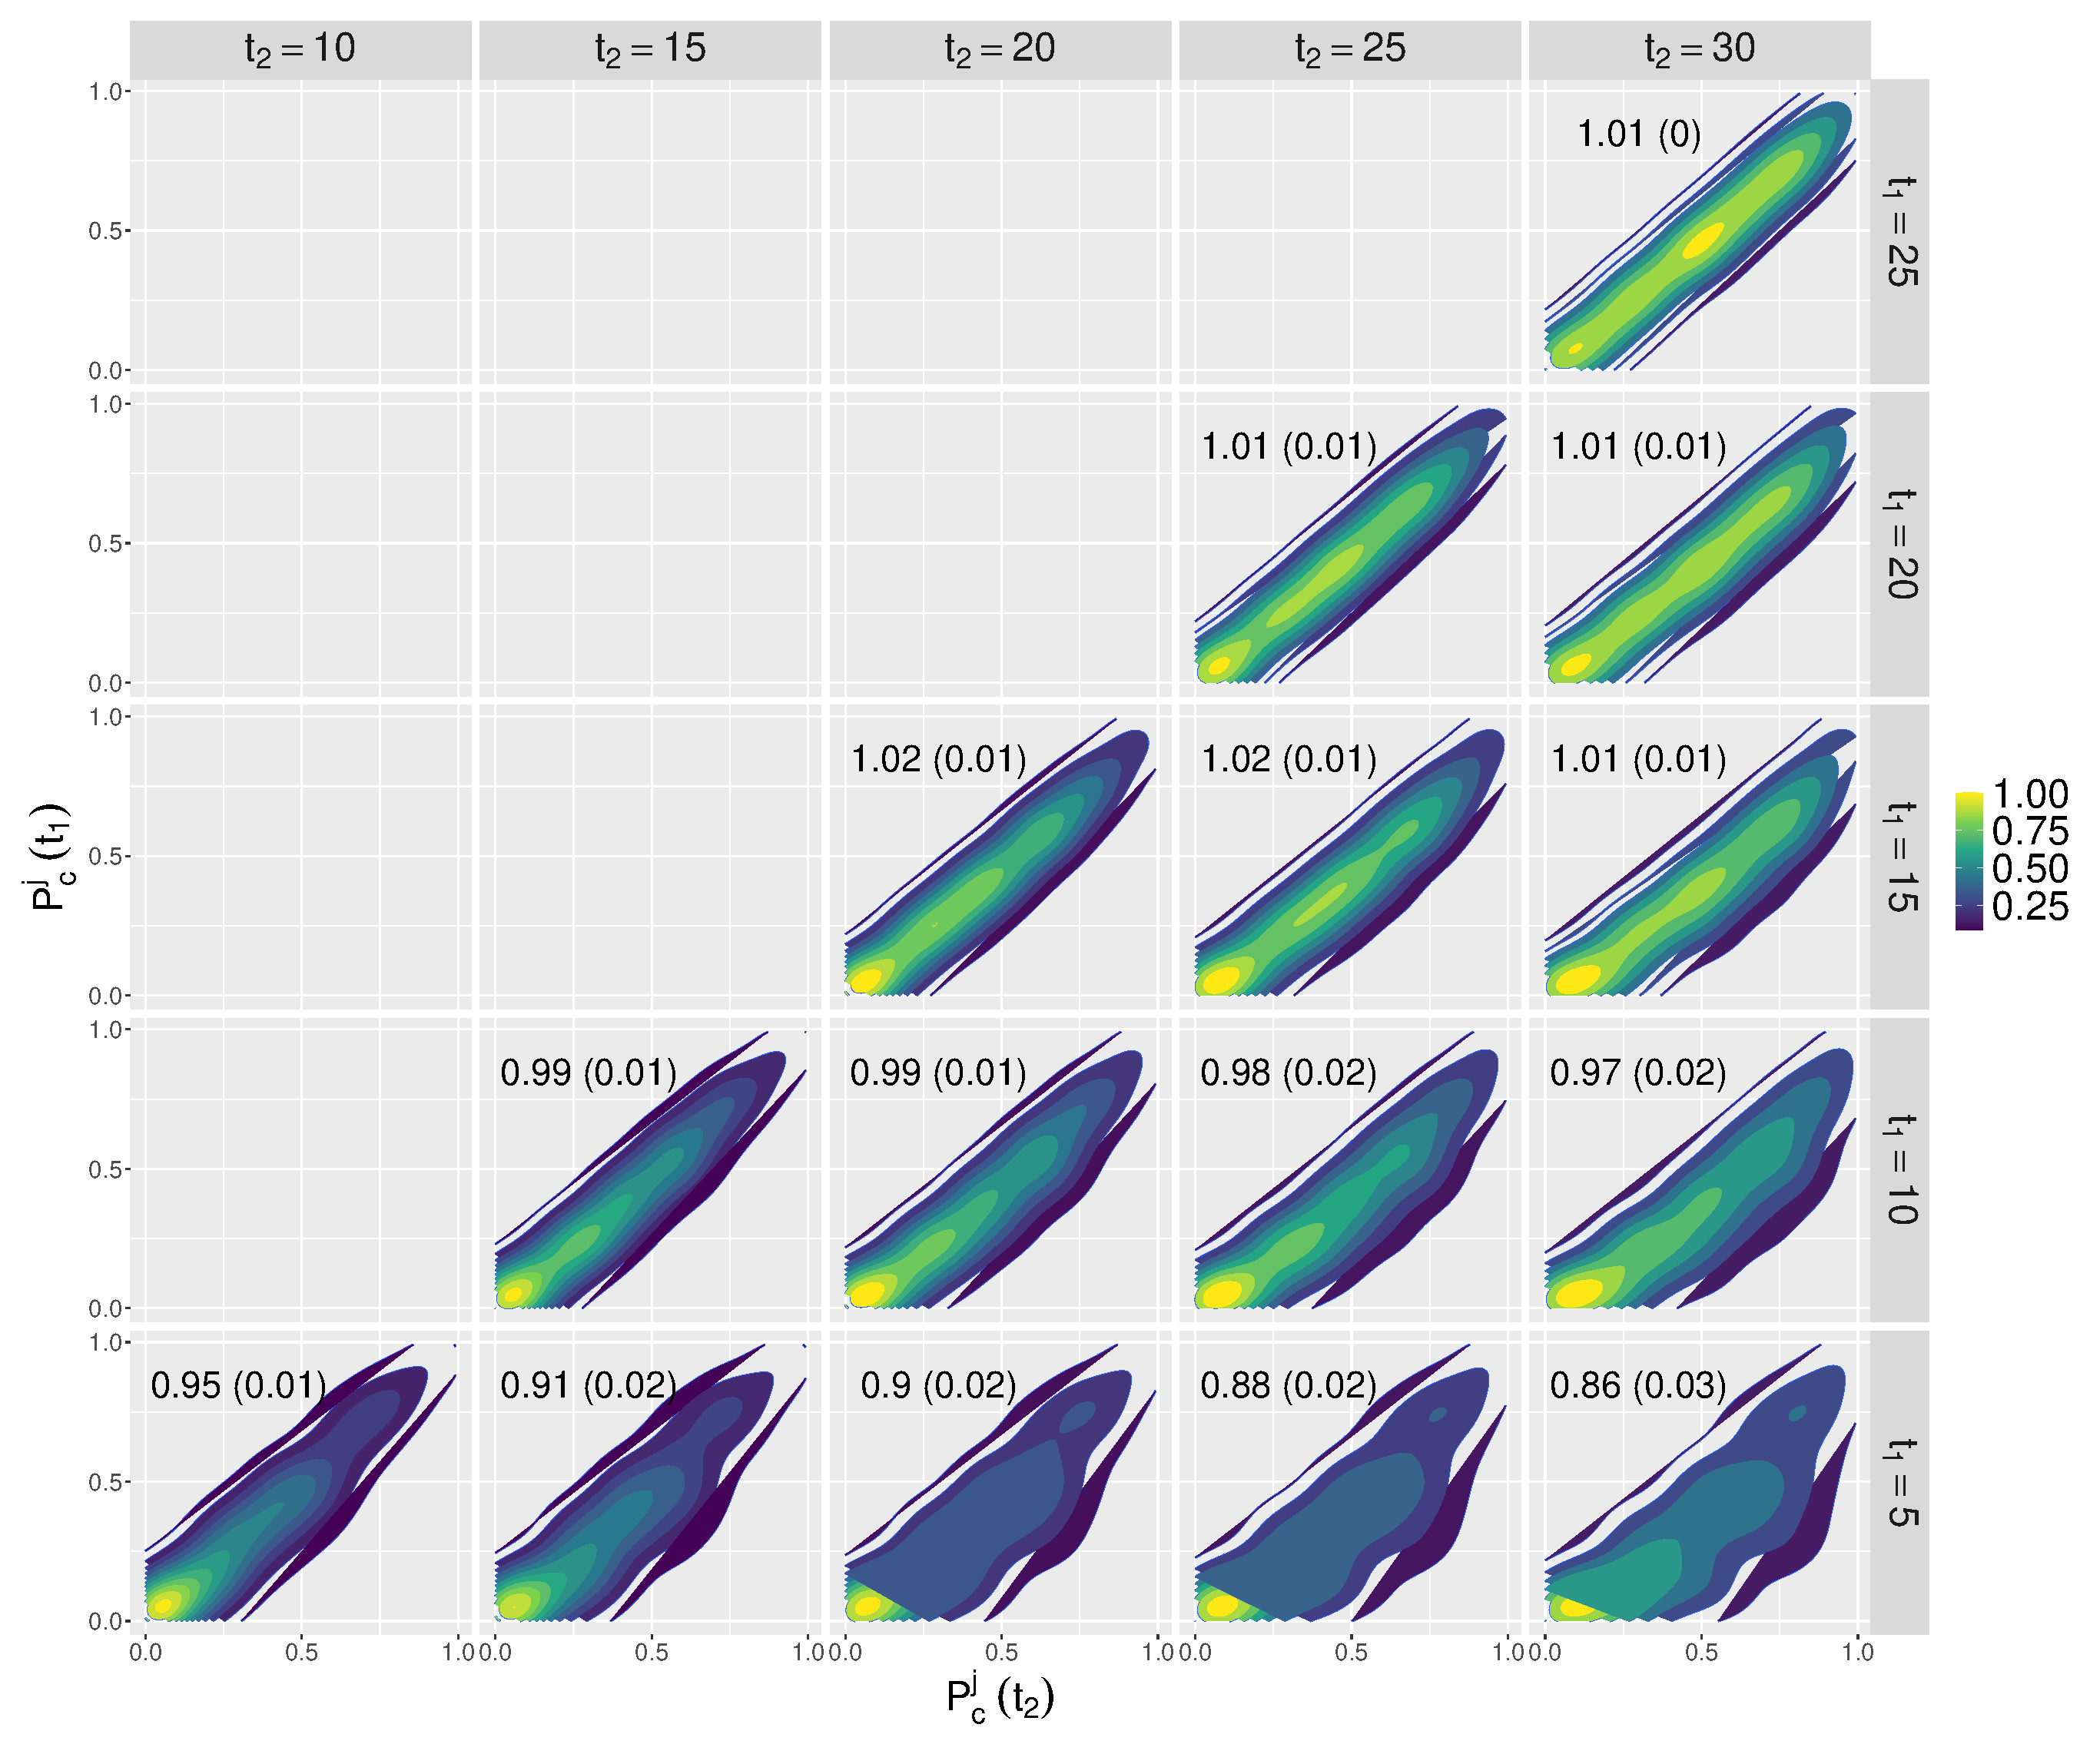
\includegraphics[width=\textwidth]{figures/pred_power/scatter_pubrp_bio1980.eps}
    \caption{{\bf Kernel Density Estimation for the Scatter Points of P$_c^j(t_1)$ and P$_c^j(t_2)$.}
    A simple linear regression of P$_c^{j}(t_2)$ on P$_c^{j}(t_1)$ is fitted. The estimated coefficient and the corresponding standard error (in parentheses) are displayed in each plot. The benchmark contains publications in biology that were published in $1980$.}
    \label{fig:scatter_pubrp_bio1980}
\end{figure}

Predicting S$_{P5}^{i}(t_2)$ can assist in decision-making for faculty positions or granting tenure, since the committee prefers to examine the cumulative scientific impact of the scholar. Committees assign research funding or allocate research resources regarding planned studies and potential future publications; consequently, the future impact of future works is often of interest. We utilized S$_{P5}^{i}(t_2|t_1)$ to denote the rank percentile indicator; this was calculated based on papers published between $t_1$ and $t_2$. Figure \ref{fig:hm_rp_aut_future} illustrates the correlation between S$_{P5}^{i}(t_1)$ and S$_{P5}^{i}(t_2|t_1)$. The magnitudes of correlation are moderately high, indicating an approximately linear relationship, although the strength is less pronounced than it was in predicting the cumulative impact, that is, predicting S$_{P5}^{i}(t_2)$, which is consistent with our expectations.

A factor causing the difficulty in predicting the future impact of future works is the different stages of a scholar's career. The first 5 years are typically when a scholar conducts their doctoral study and begins research under supervisions. The next 5 years of their academic career typically includes a postdoctoral study or an assistant professorship, in which the productivity and quality of works usually improve over those from the first 5 years, thus resulting in relatively low correlation (the value is $0.65$, according to Figure \ref{fig:hm_rp_aut_future}) between S$_{P5}^{i}(5)$ and S$_{P5}^{i}(10|5)$. As the scholar earns seniority and produces a more consistent stream of publications, the discrepancy between different stages of their career becomes less discernible. For instance, the correlation increases to $0.7$, when $t_1=10$ and $t_2=15$. 

\subsection*{Predictive Models}

In this section, we formulate the prediction tasks as supervised learning problems, and we illustrate that the rank percentile indicators can be predicted via simple linear models. We consider the following fitting procedures; these models are ordered by increasing complexity:
\begin{itemize}
    \item Baseline: simple linear regression model.
    \item Simple Markov model (sm).
    \item Penalized linear regression models, including the ridge~\cite{hoerl1970ridge}, lasso~\cite{Tibshirani1996}, elastic net (enet)~\cite{zou2005regularization} and the Gamma lasso (gamlr)~\cite{Taddy2017}.
    \item Ensemble methods of regression trees, including the random forest (rf)~\cite{liaw2002classification} and extreme gradient boosting trees (xgbtree)~\cite{chen2016xgboost}.
    \item Neural networks (nnet).
\end{itemize}

Recall that the three prediction tasks discussed in the above section are predicting the future impact of publication percentile, the future impact of scholar percentile, and the future impact of scholar percentile based on futuer works, where the target variables are P$_c^j(t_2)$, S$_{P5}^i(t_2)$, and S$_{P5}^i(t_2|t_1)$, respectively. The baseline model fits a simple linear regression of the target variable on the autoregressive feature, such as P$_c^{j}(t_1)$ for predicting the publication impact. The simple Markov model further considers the change of the autoregressive feature in the past two ages, for instance P$_c^{j}(t_1)$-P$_c^{j}(t_1-2)$, in addition to the autoregressive feature; furthermore, it fits a linear regression model. 

\subsubsection*{Features and Model Fitting}

For the remainder of the methods, we created an extensive list of features based on the citation histories. The features were characterized as either scholar- or publication-based features. For example, to predict the scholar indicator S$_{P5}^{i}(t_2)$, a scholar-based feature is the number of papers that scholar $i$ publishes by age $t_1$, and a publication-based feature is the average number of citations for these papers. We established $30$ features for predicting the publication indicator and $42$ features for predicting the scholar indicator, which can be found in the Supplemental Material Tables \ref{tab:features_pubrp} and \ref{tab:features_autrp}, respectively. Note that many of the features have been utilized when formulating the prediction task for number of citations and h-index scores~\cite{acuna2012future,weihs2017learning,weis2021learning}.

The features were created utilizing the citation information available via $t_1$, and the dependent variable was specified at $t_2$. We considered five stages of a publication or a scholar: $t_1\in\{5,10,15,20,25\}$, and we forecasted through $30$ years of age: $t_2=t_1+1,\cdots,30$; this resulted in $75$ pairs of $(t_1,t_2)$ in total. Every model was trained $75$ times, once for each pair of $(t_1,t_2)$.

The rank percentiles were calculated utilizing all the publications and scholars in the dataset. We then restricted data for the prediction task to maintain the same set of publications and scholars for the entire forecast horizon (up to 30 years). To predict the publication impact, we employed a subset of data by including papers with more than $30$ years of age, which corresponds to papers published before 1987, since the most recent year considered in the dataset is 2016; this resulted in $36,372$ papers. Similarly, for the scholar impact prediction task, we utilized scholars who started their careers before 1987; this resulted in $1,457$ scholars. 

We also noted (in the Supplemental Material Section \ref{sec:suppl_stationarity}) that both S$_{P5}$ and P$_c$ were non-stationary time series, as evidenced by the Dicky-Fuller test~\cite{dickey1979distribution} and the KPSS test~\cite{kwiatkowski1992testing}. The differenced series were stationary (also presented in the Supplemental Material) and were utilized as the response variables: $\Delta \text{P}_{c}^{j}(t_2) = \text{P}_{c}^{j}(t_2) - \text{P}_{c}^{j}(t_1)$, $\Delta \text{S}_{P5}^{i}(t_2) = \text{S}_{P5}^{i}(t_2) - \text{S}_{P5}^{i}(t_1)$, and $\Delta \text{S}_{P5}^{i}(t_2|t_1) = \text{S}_{P5}^{i}(t_2|t_1) - \text{S}_{P5}^{i}(t_1)$. Note that the stationarity discussed here characterizes the property of S$_{P5}$ and P$_c$ as time series. It is different from the stationarity as discussed in Figure \ref{fig:rp_stationarity}, in which we fixed $t=10$ and examined the stationarity of S$_{P5}(10)$ over the starting year of the scholars' careers.

The machine learning methods were trained in \textit{R}~\cite{RCT2019} utilizing the package \textit{mlr}~\cite{Bischl2016}, which provides a pipeline of training, validating, and testing for the model. The lasso, ridge, elastic net, random forest, and xgbtree modles are built into the package. The Gamma lasso and neural network were trained utilizing \textit{R} packages \textit{gamlr}~\cite{Taddy2017} and \textit{keras}~\cite{Allaire2019}, respectively. 

The machine learning methods require hyperparameter tuning, which involves deciding the search space of parameters and evaluating the sets of parameters utilizing the validation data. The hyperparameters for each machine learning model considered in this paper are presented in the Supplemental Material Table \ref{tab:hyperpara}. Each hyperparameter has a grid of predefined values, and the search space is the combination of all parameters. The parameter space can be substantial for methods such as xgbtree and nnet, which utilize extensive lists of tunable parameters. For these methods, we applied Bayesian optimization, which searches over the parameter space based on the performance gain. The optimal choice of hyperparameters is that which minimizes the validation error, where a holdout validation set was utilized for xgbtree and nnet, and 10-fold cross-validation was employed for the other methods.


\subsubsection*{Performance of the predictive models}

The data were randomly split into the training and test set at a 9:1 ratio. The accuracy of prediction on the holdout test set in terms of testing $R^2$ is presented in Figure \ref{fig:pred_r2}. We see that the simple linear regression model predicted the cumulative impacts well, i.e. P$_c^{j}(t_2)$ and S$_{P5}^{i}(t_2)$, and the usage of a large number of features and complex machine learning models offered little improvement. Predicting the future impact of scholars, S$_{P5}^{i}(t_2|t_1)$, is considerably more difficult. The simple linear regression model provided reasonable predictions, but the performance was not as satisfactory as other methods, especially when $t_1$ was large. By adding the difference presented in $\text{S}_{P5}^{i}(t_1) - \text{S}_{P5}^{i}(t_1-2)$ as an extra feature, the simple Markov model achieved similar performance compared to the complex machine learning models that rely on extensive lists of features and exhibit non-linear relationships. The conclusion is robust against the choice of error measure, and we present the results utilizing the root mean squared error, root median squared error, and mean absolute error in the Supplemental Material (Figure \ref{fig:pred_rmse}, \ref{fig:pred_medse}, and \ref{fig:pred_mae}, respectively). 

\begin{figure}[ht!]
    \centering
    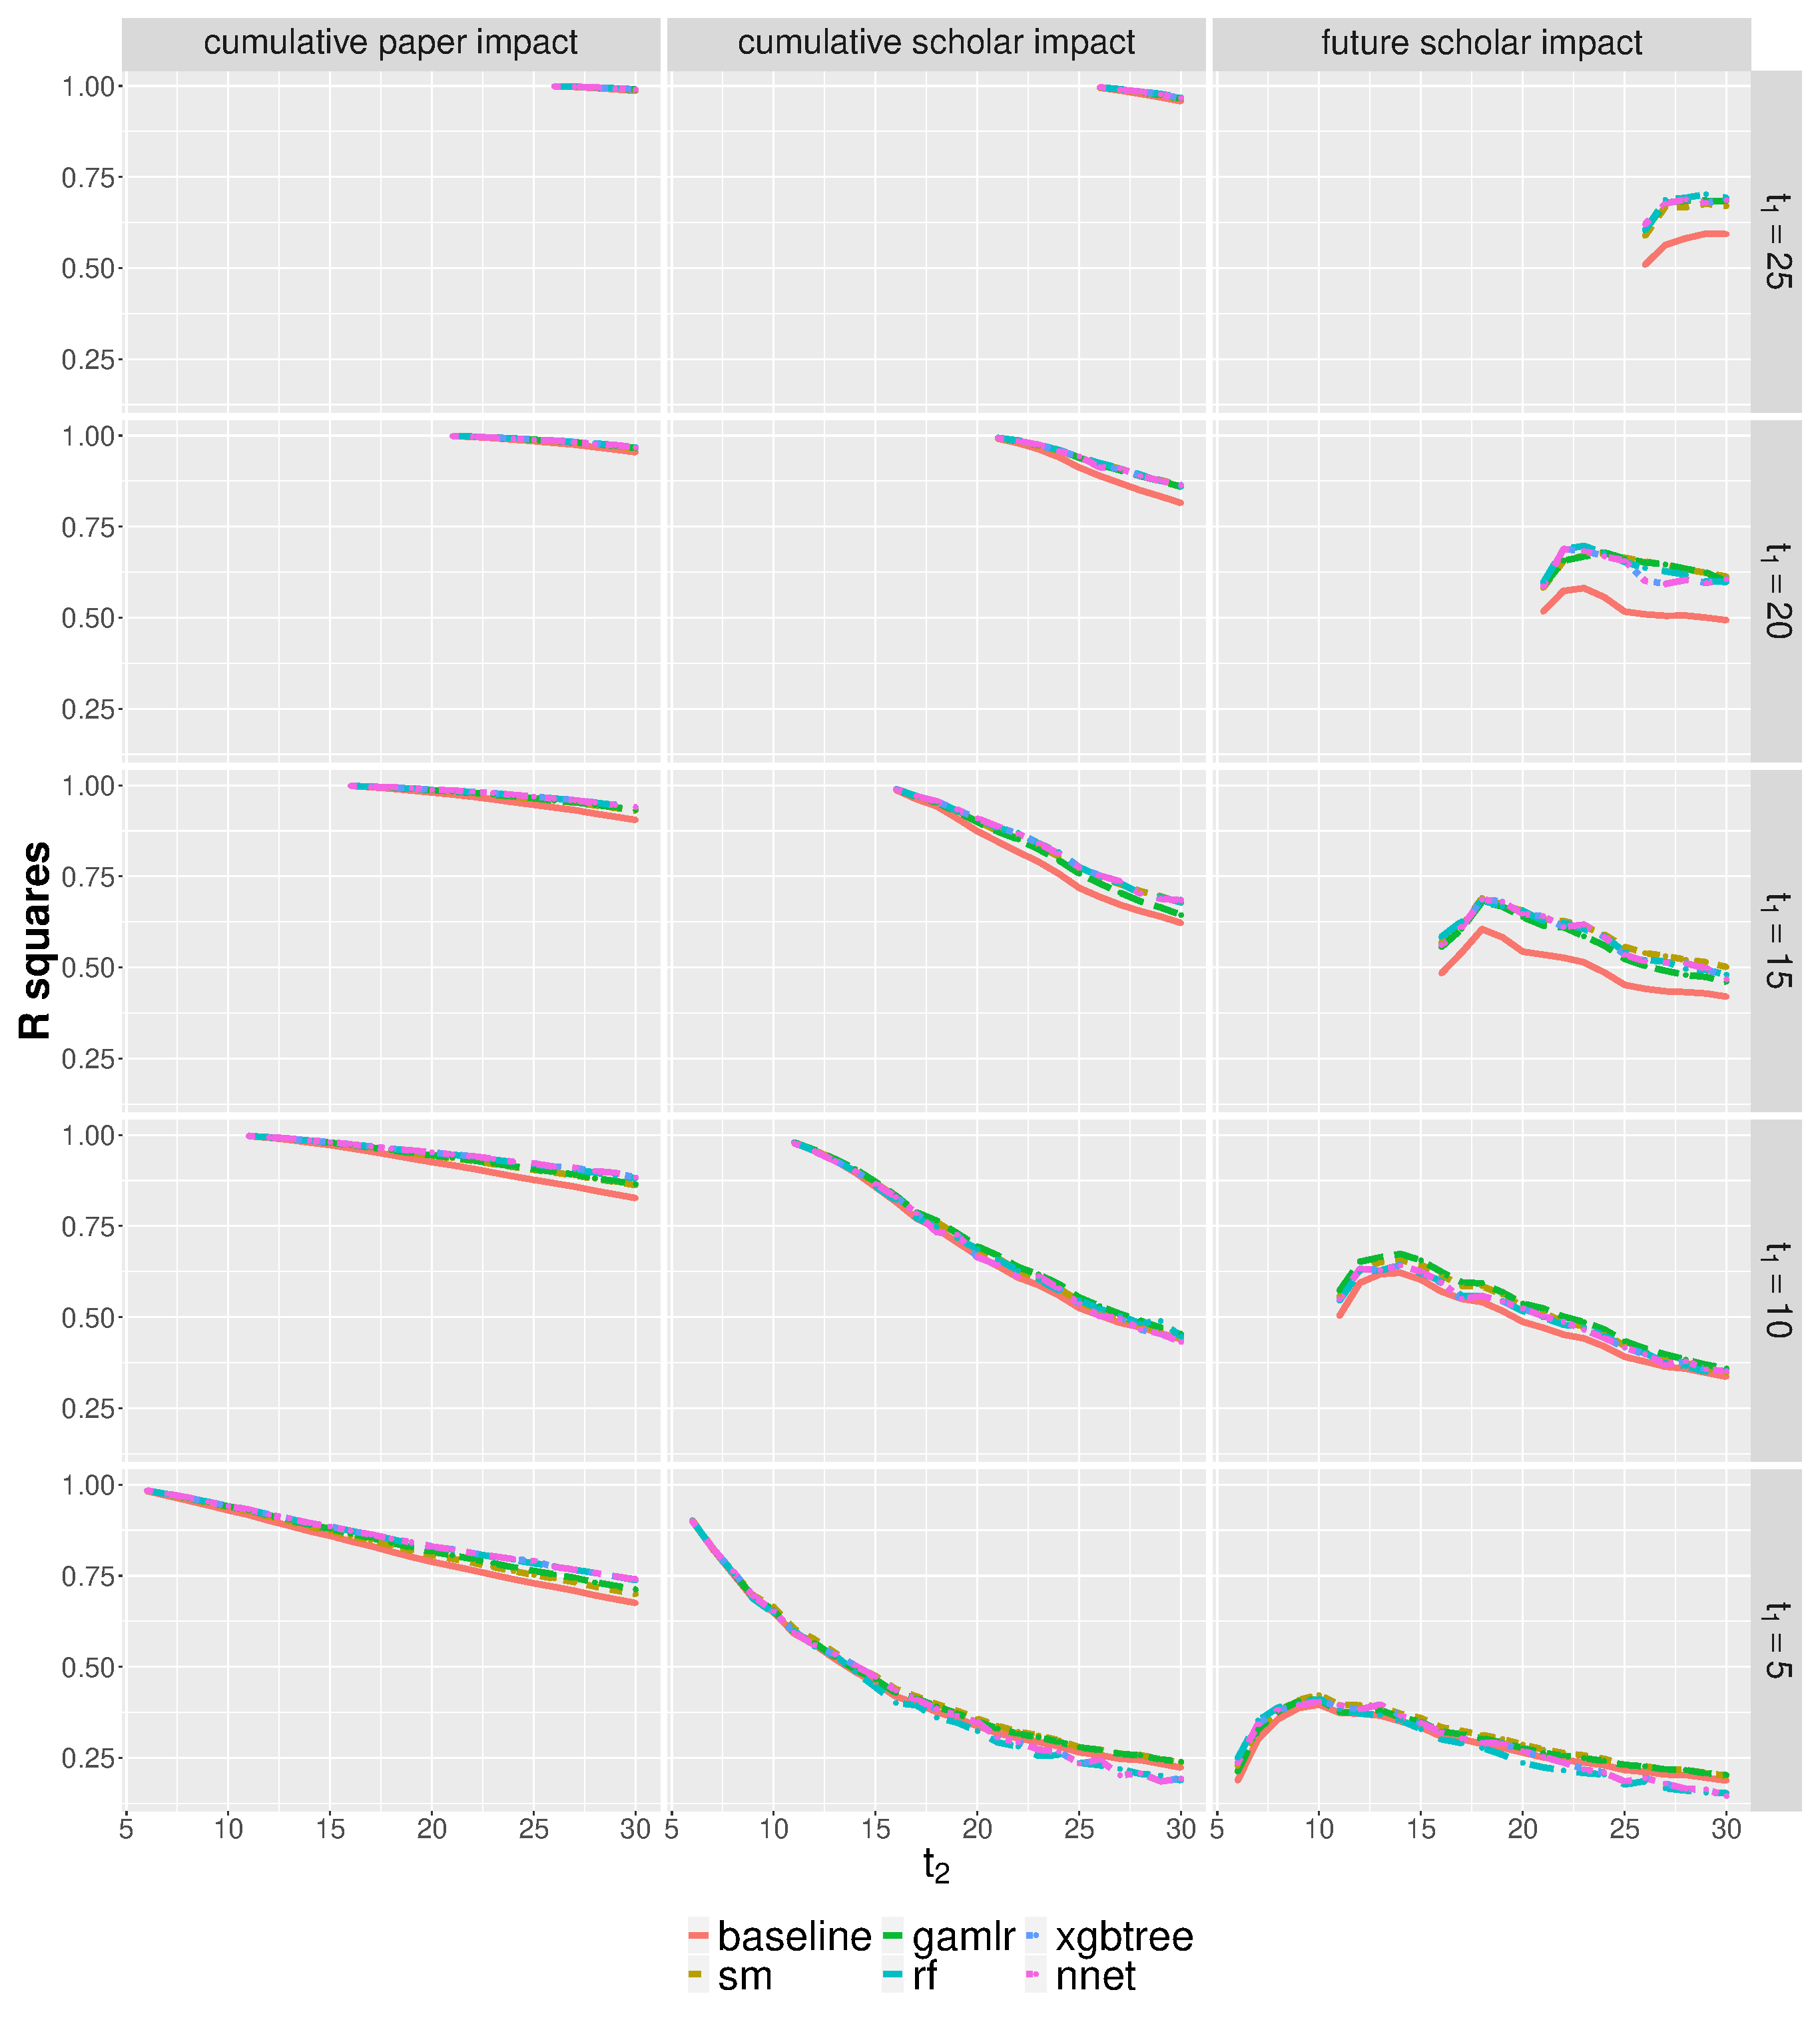
\includegraphics[width=\textwidth]{figures/pred_model/r2.eps}
    \caption{{\bf Testing $R^2$ for the Predictive Models.} The target variables, from left to right panel, are P$_c^{j}(t_2)$, S$_{P5}^{i}(t_2)$, and S$_{P5}^{i}(t_2|t_1)$, respectively. The lasso, ridge, and elastic net are outperformed by the Gamma lasso, and hence are ignored for a better visualization.}
    \label{fig:pred_r2}
\end{figure}


The overall patterns in Figure \ref{fig:pred_r2} matches those in Figure \ref{fig:hm_rp}. To predict the cumulative impact, we observe that the overall $R^2$ becomes larger as $t_1$ increases and the $R^2$ decreases as the forecast horizon increases. An interesting pattern that we did not observe previously (since the smallest forecast horizon in Figure \ref{fig:hm_rp} was $5$ years) is that for predicting the future scholar impact, the $R^2$ curves exhibit non-monotonic shapes. For instance, when $t_1=5$, the $R^2$ increases from approximately $0.25$ ($t_2=6$) to $0.5$ ($t_2=10$) before decreasing. A scholar's first 5-year performance is not necessarily a quality indicator for the 6th-year performance, potentially due to external factors, such as the processing time of journals, which can be anywhere from months to years depending on the culture, quality of the venue, field, and availability of referees. Hence, a promising scholar may experience a publication drought in the 6th year simply because the submitted papers take longer than usual to be reviewed; this causes S$_{P5}^{i}(5)$ to be a poor indicator for S$_{P5}^{i}(6|5)$. The effect of the external factors diminishes as we allow a longer horizon ($t_2-t_1$) for the evaluation, and therefore we notice an increase of $R^2$ when $t_2$ becomes $10$. As $t_2$ further increases, the difficulty of long-term forecasting enters, and the $R^2$ decreases.





